
\chapter[Systematic uncertainties for signal]{Systematic uncertainties across the T1ttcc
(\texorpdfstring{$\mathbf{\Delta m = 25}\GeV$}{Dm=25GeV}) mass plane 
\label{app:signal_systematics}}

In the section on systematic uncertainties, in Table~\ref{tab:bgsigsys}, we presented the average of
the systematic effects across the signal mass plane. Here, in Figs.~\ref{fig:sig_sys_1} to
\ref{fig:sig_sys_end}, we show the one standard deviation ($\sigma$) up and down variations of the
considered signal systematics for each point in the ($m_{\tilde{g}}$,$m_{\lsp}$) plane. 

\vspace{1eM}

\begin{figure}[htpb]
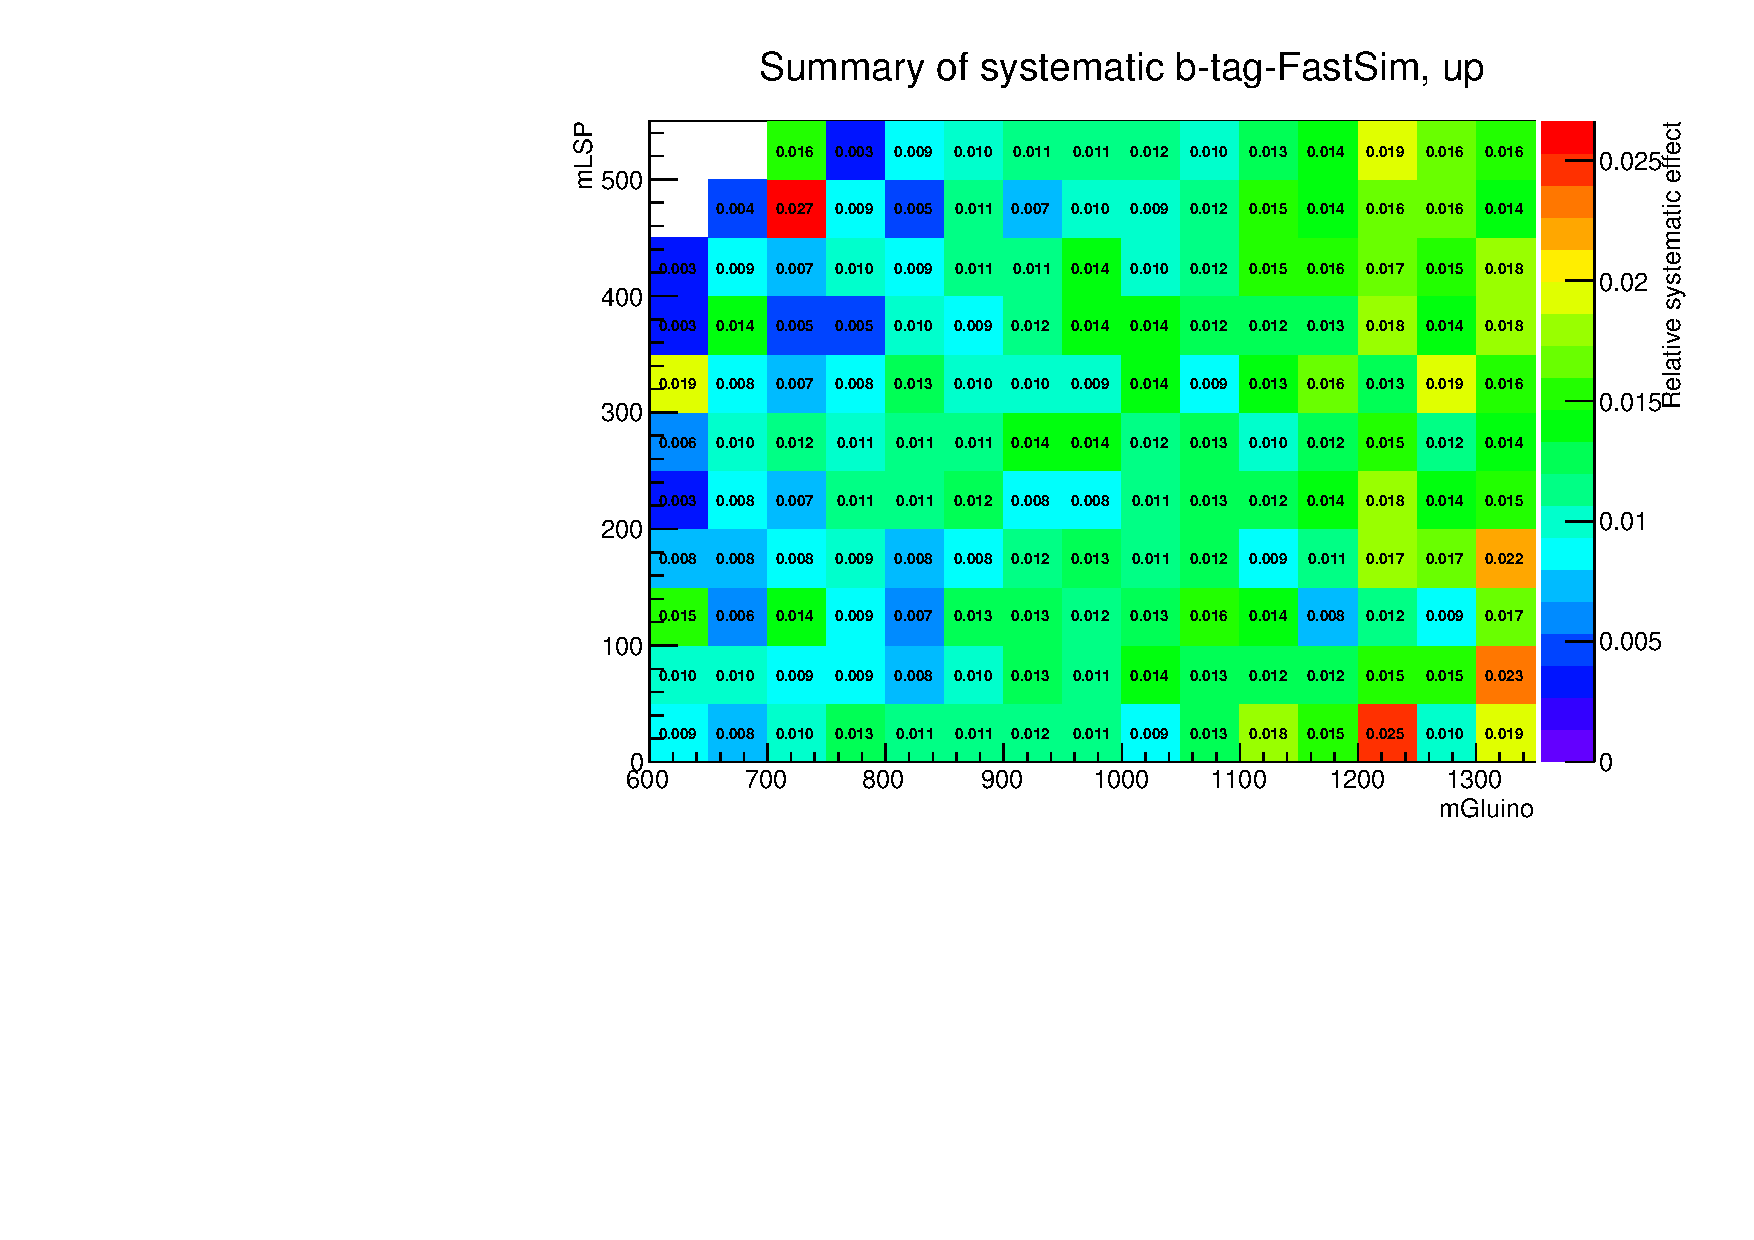
\includegraphics[width=0.49\textwidth]{figures/app_sig_syst/sys_b-tag-FastSim_up}
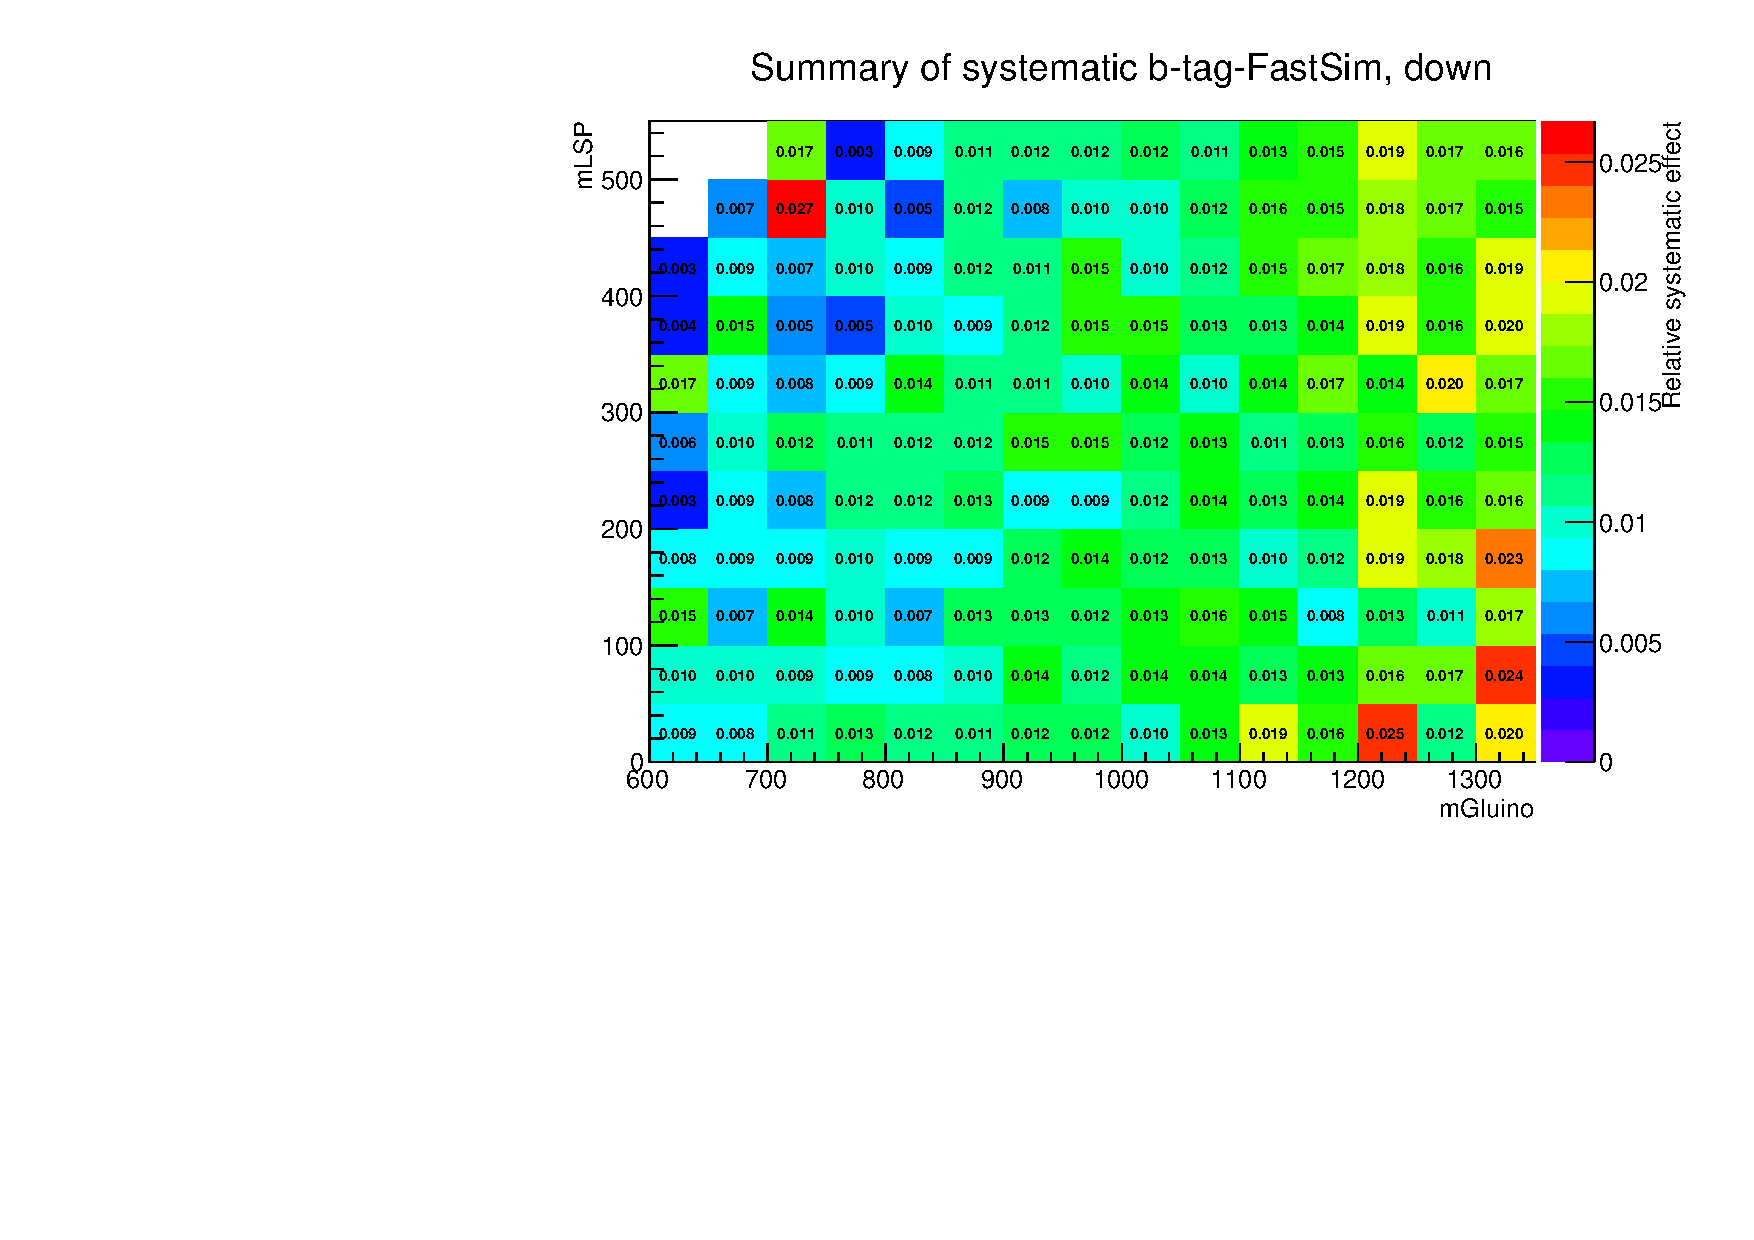
\includegraphics[width=0.49\textwidth]{figures/app_sig_syst/sys_b-tag-FastSim_down}
\caption{$1\sigma$ up (left) and down (right) variation for $\cPqb$ tag FullSim/Fastsim SF.
\label{fig:sig_sys_1}}
\end{figure}

\begin{figure}[htpb]
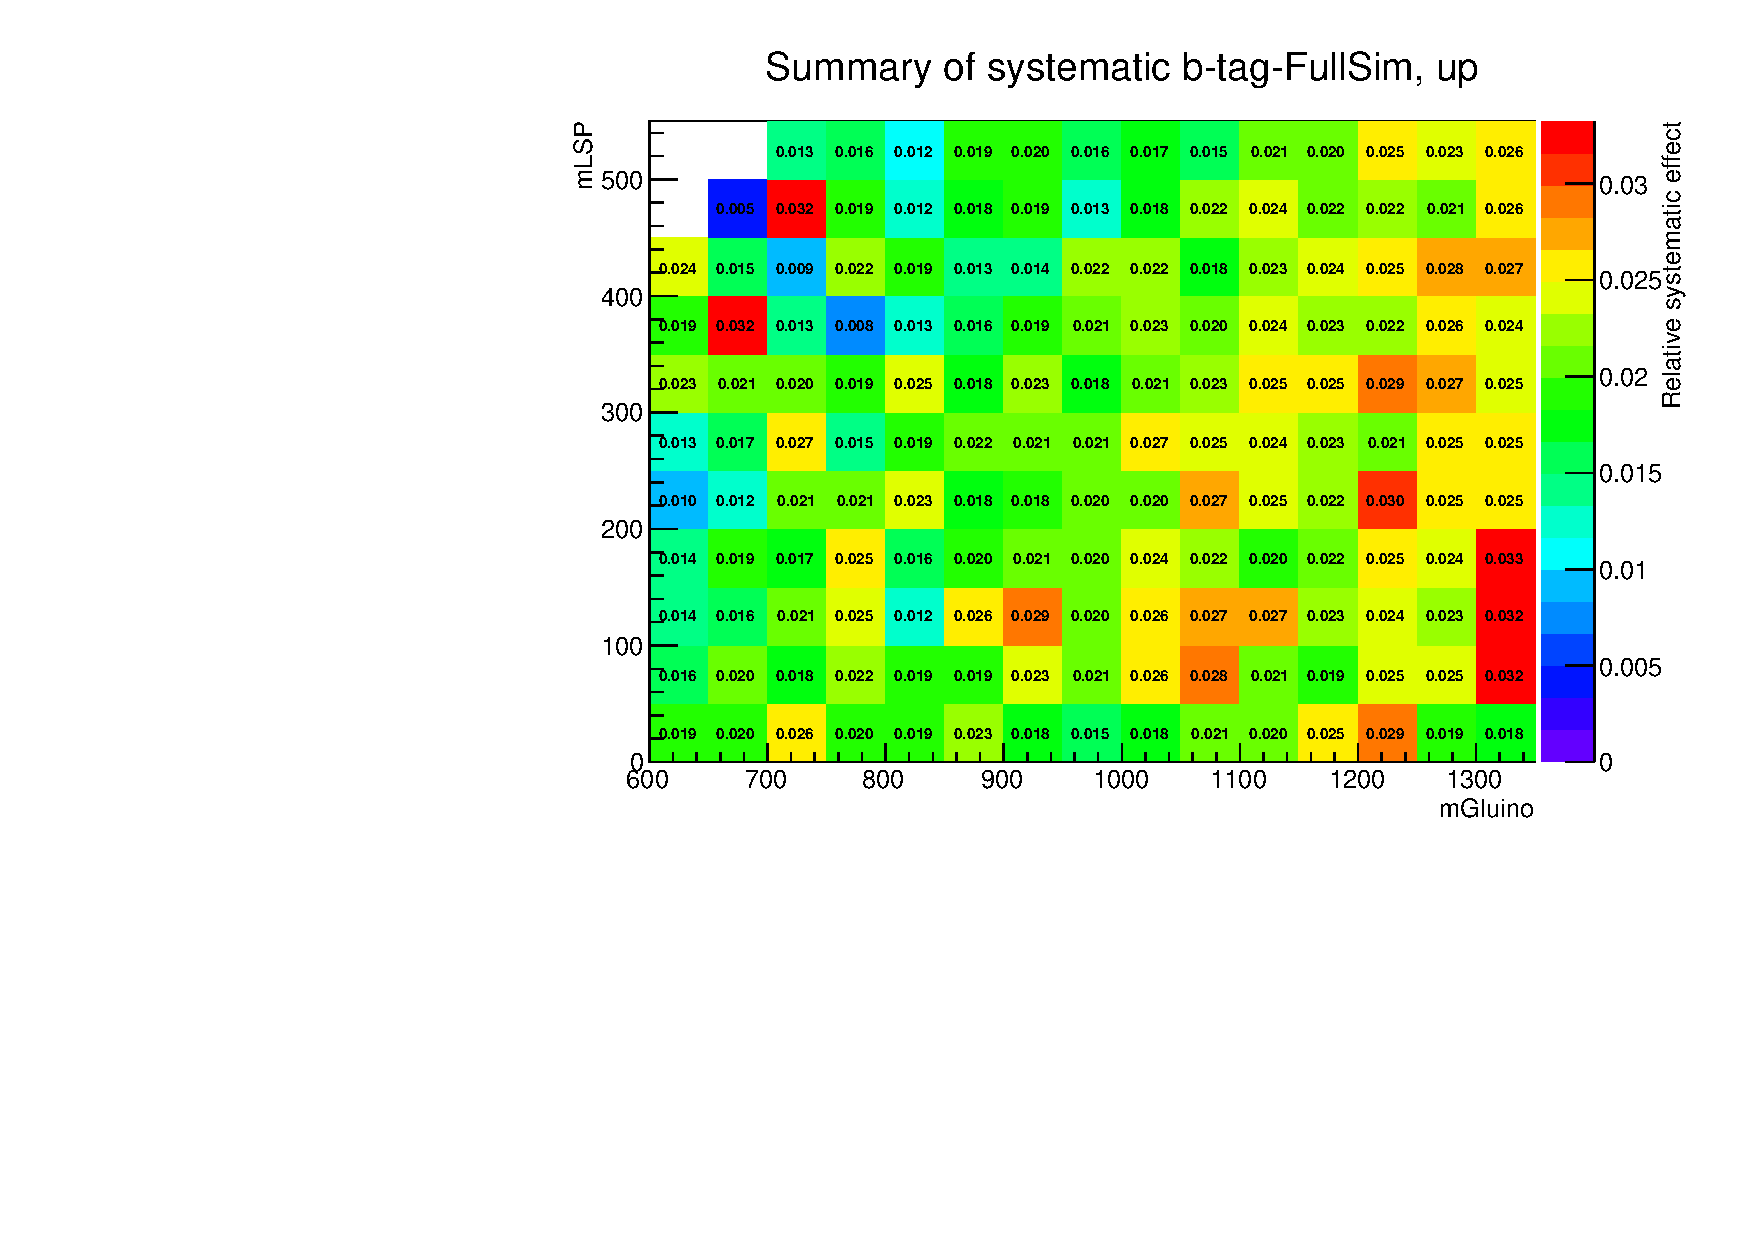
\includegraphics[width=0.49\textwidth]{figures/app_sig_syst/sys_b-tag-FullSim_up}
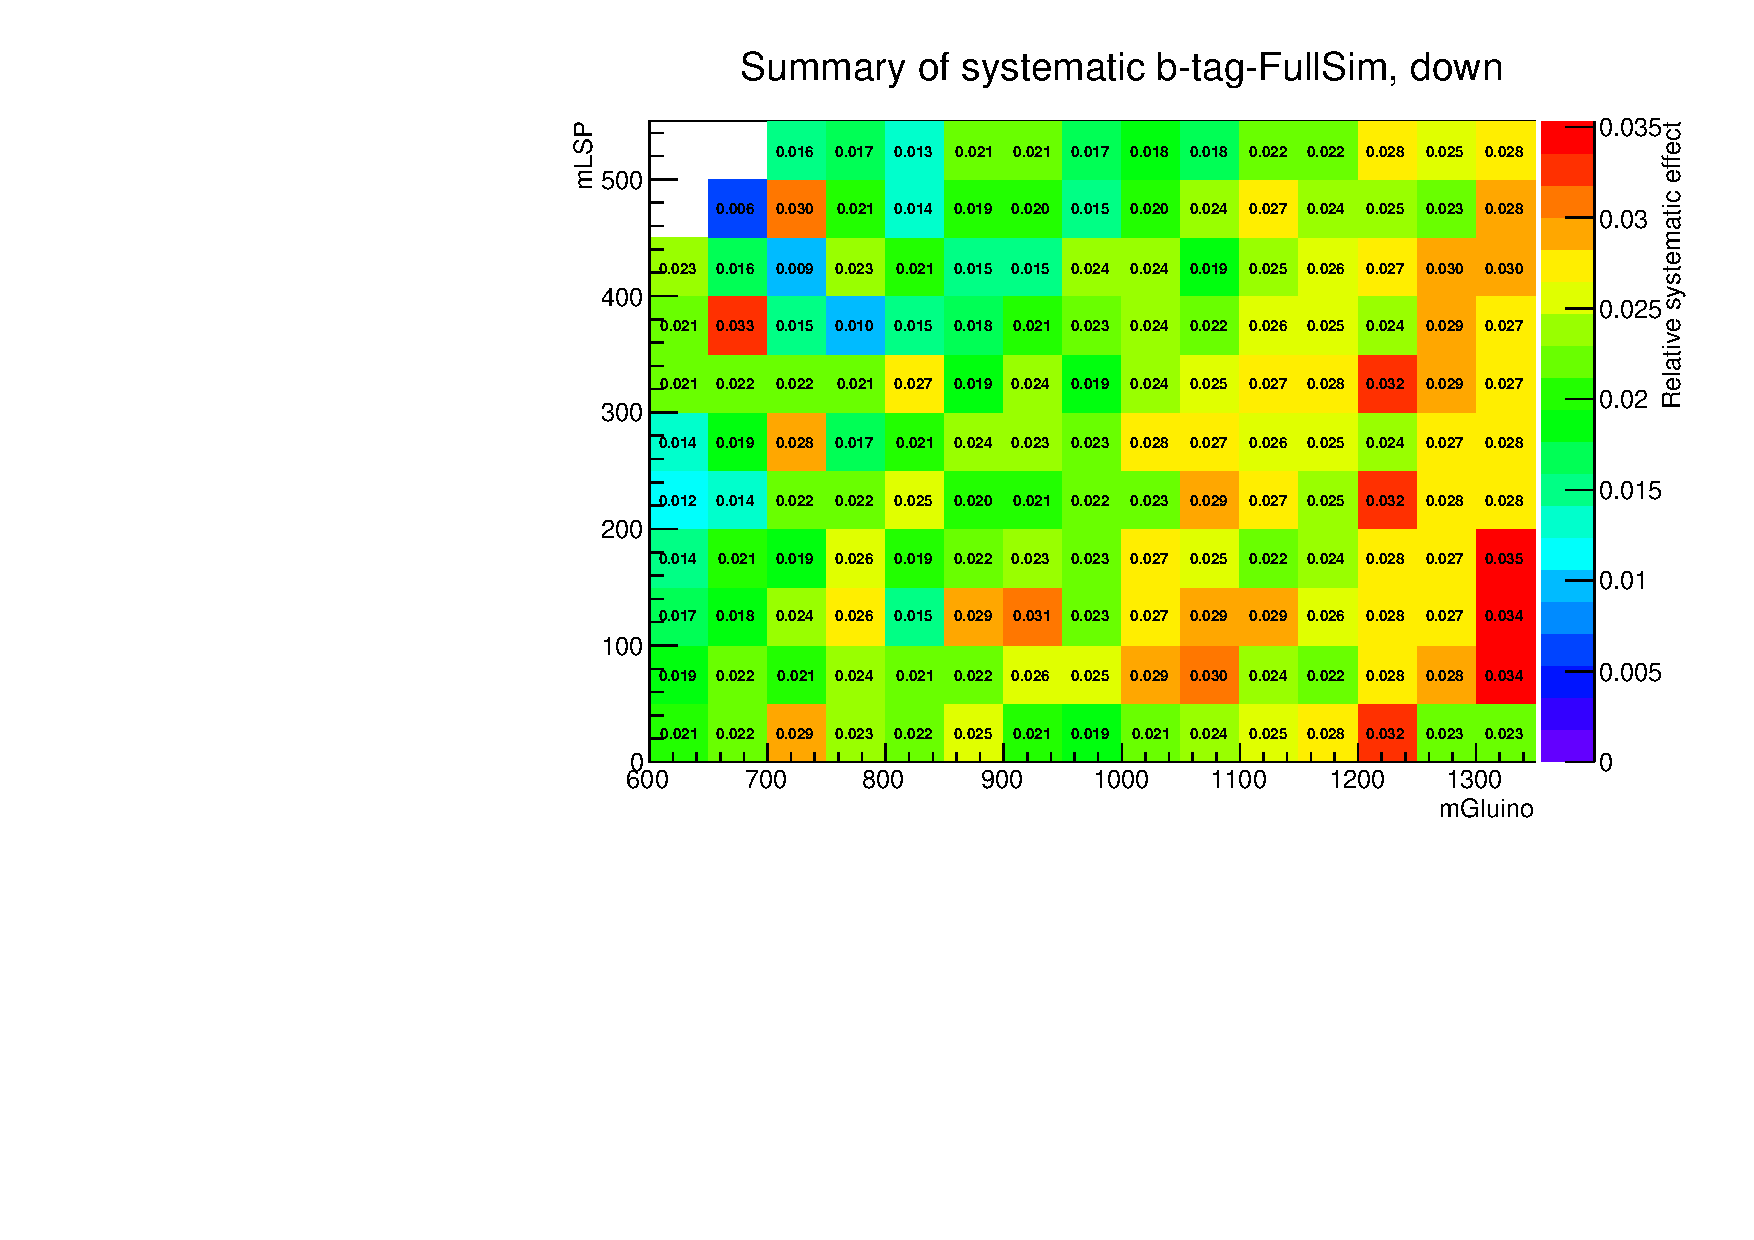
\includegraphics[width=0.49\textwidth]{figures/app_sig_syst/sys_b-tag-FullSim_down}
\caption{$1\sigma$ up (left) and down (right) variation for $\cPqb$ tag Data/FullSim SF.}
\end{figure}

\begin{figure}[htpb]
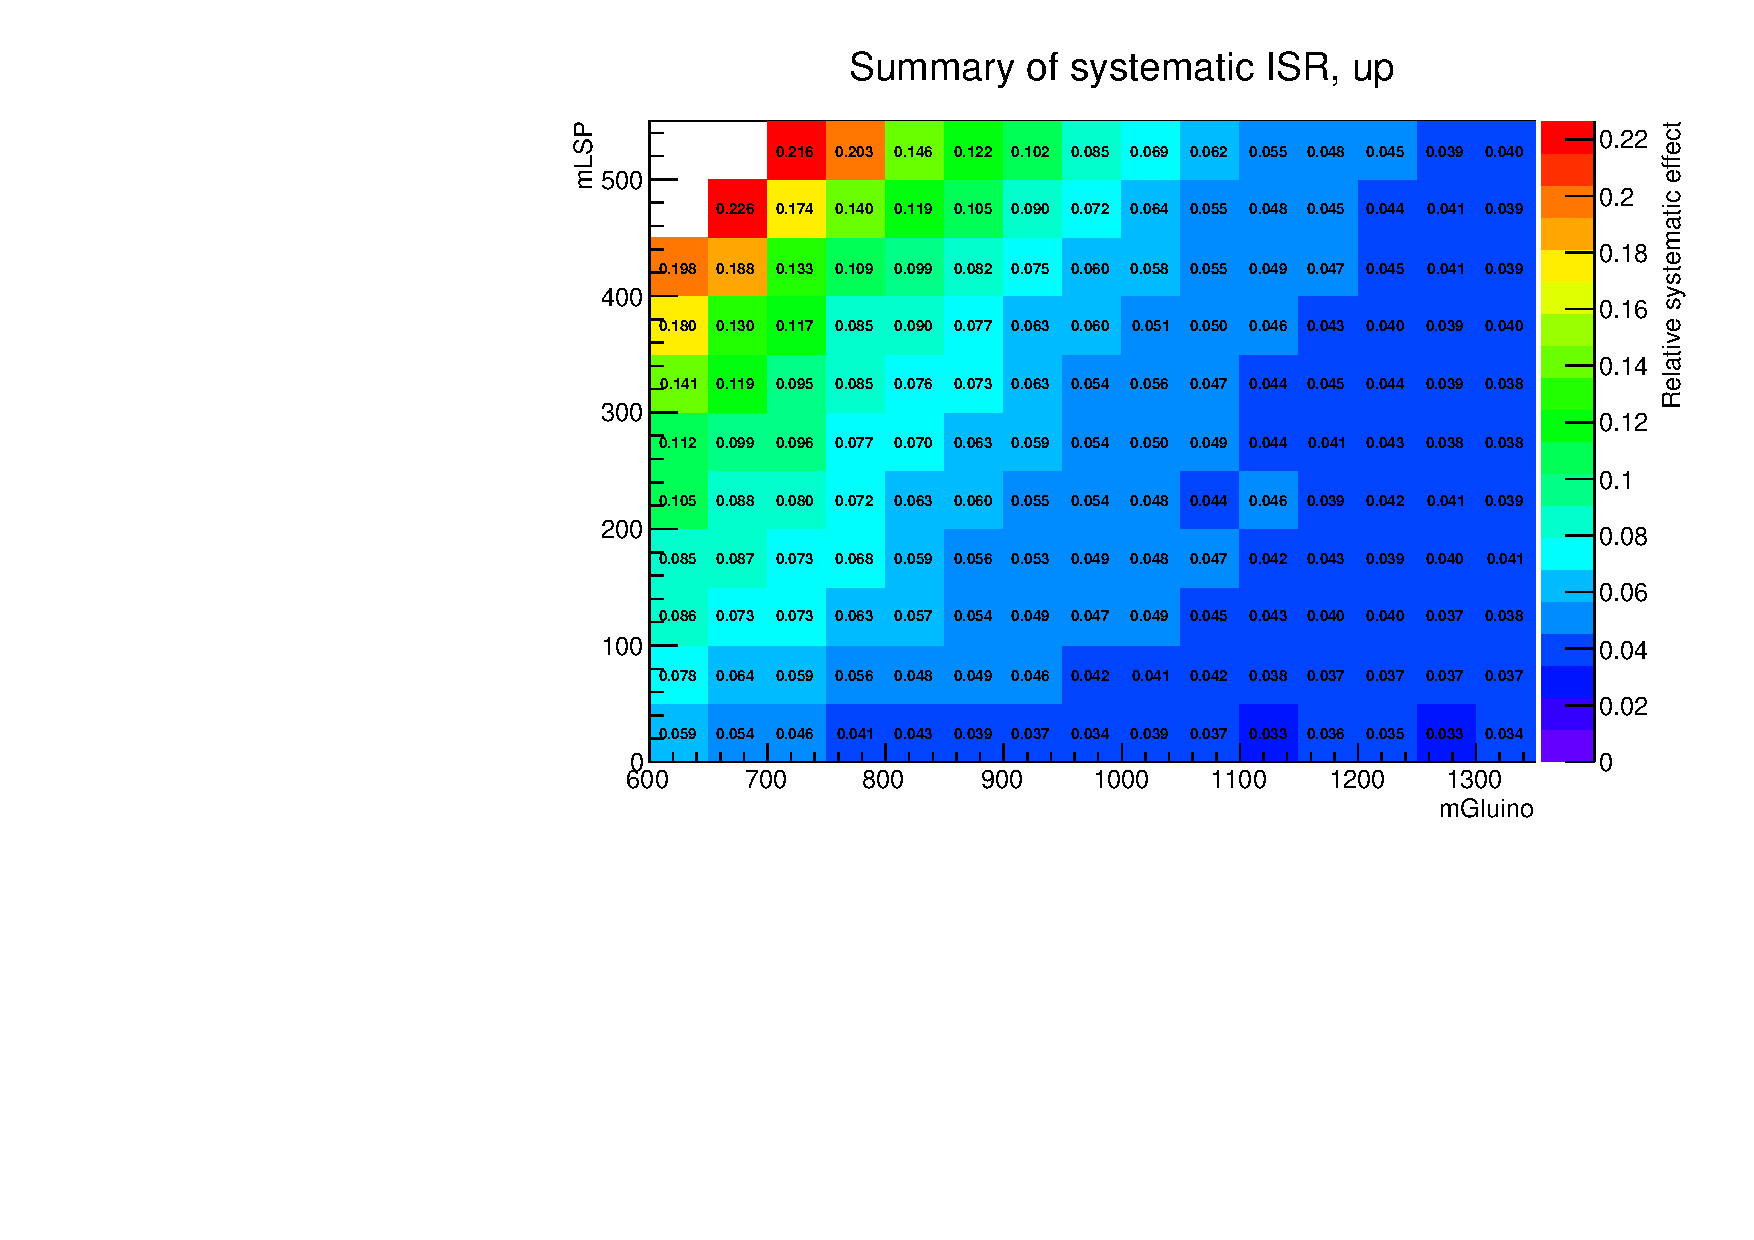
\includegraphics[width=0.49\textwidth]{figures/app_sig_syst/sys_ISR_up}
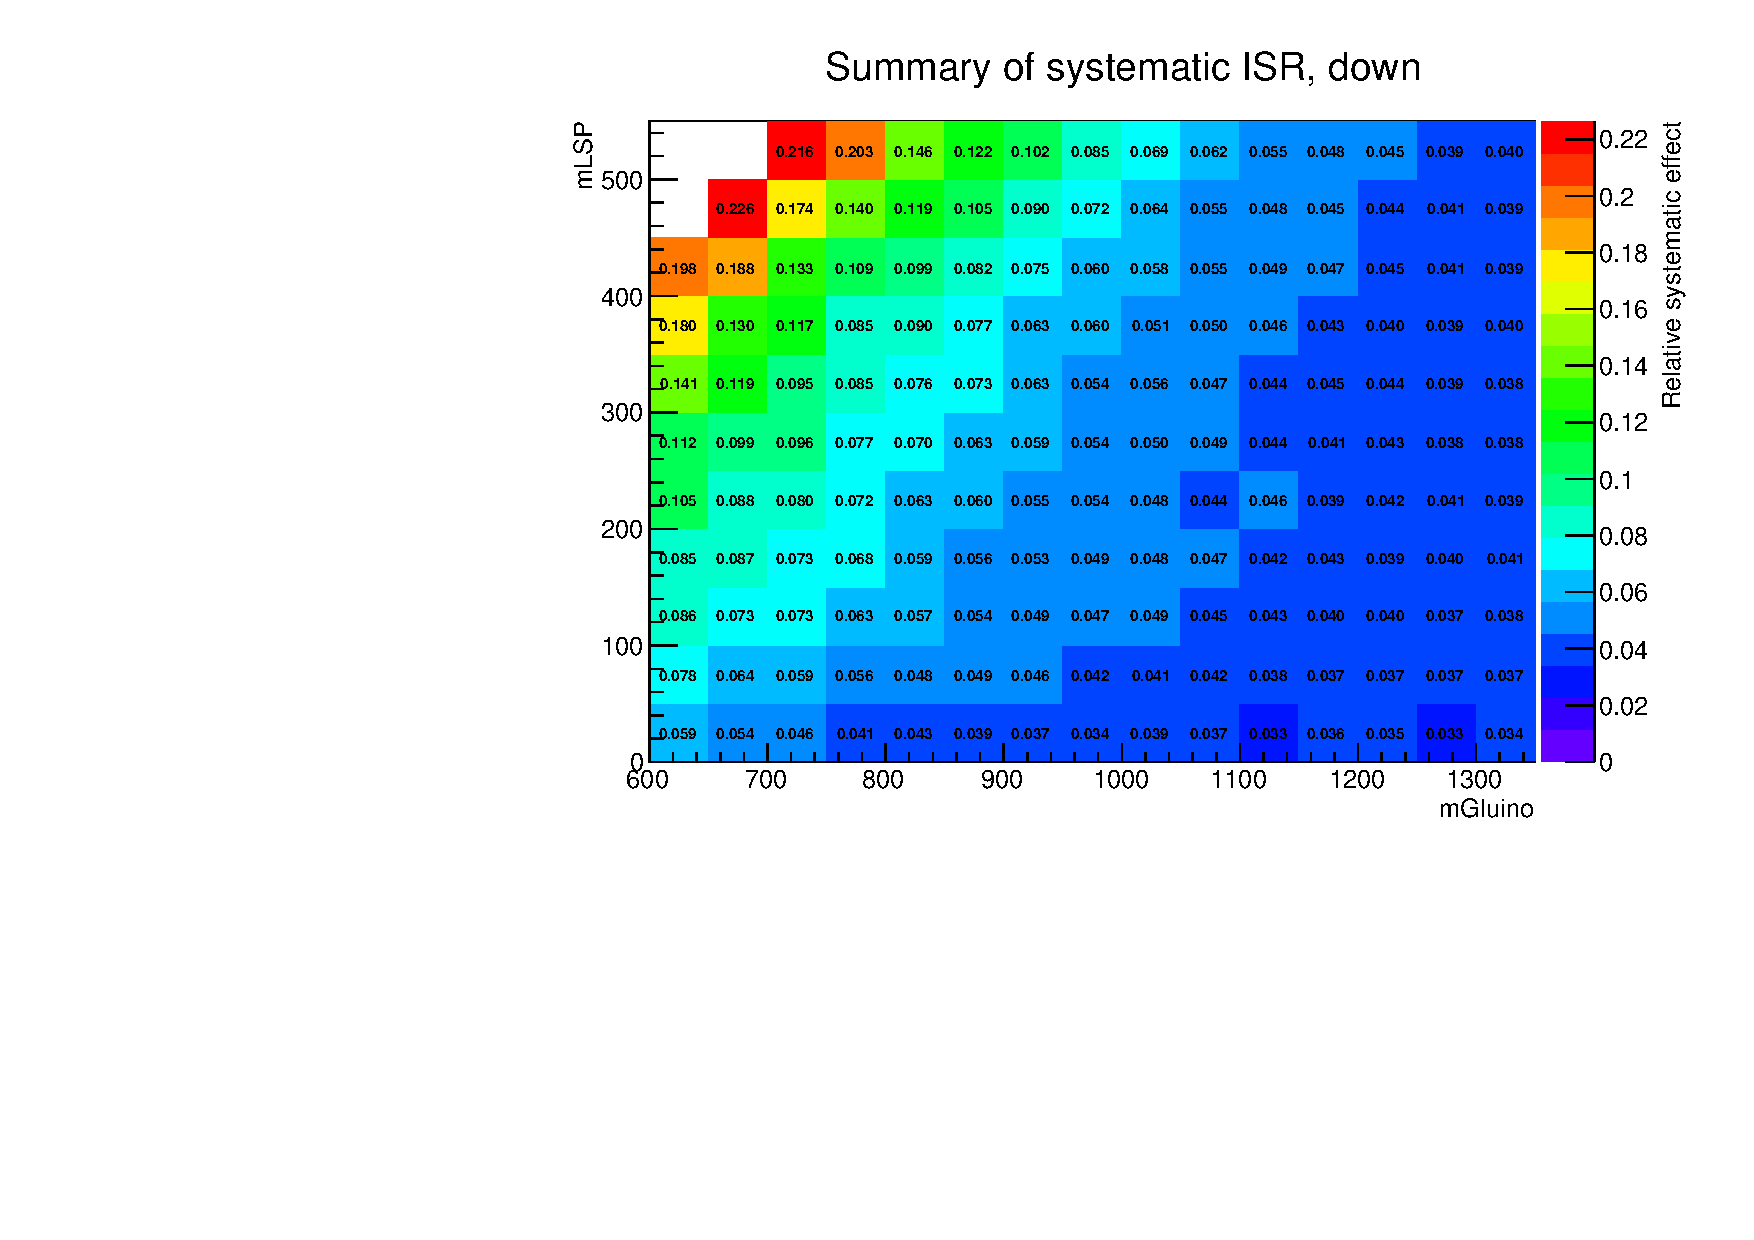
\includegraphics[width=0.49\textwidth]{figures/app_sig_syst/sys_ISR_down}
\caption{$1\sigma$ up (left) and down (right) variation for ISR reweighting.}
\end{figure}

\begin{figure}[htpb]
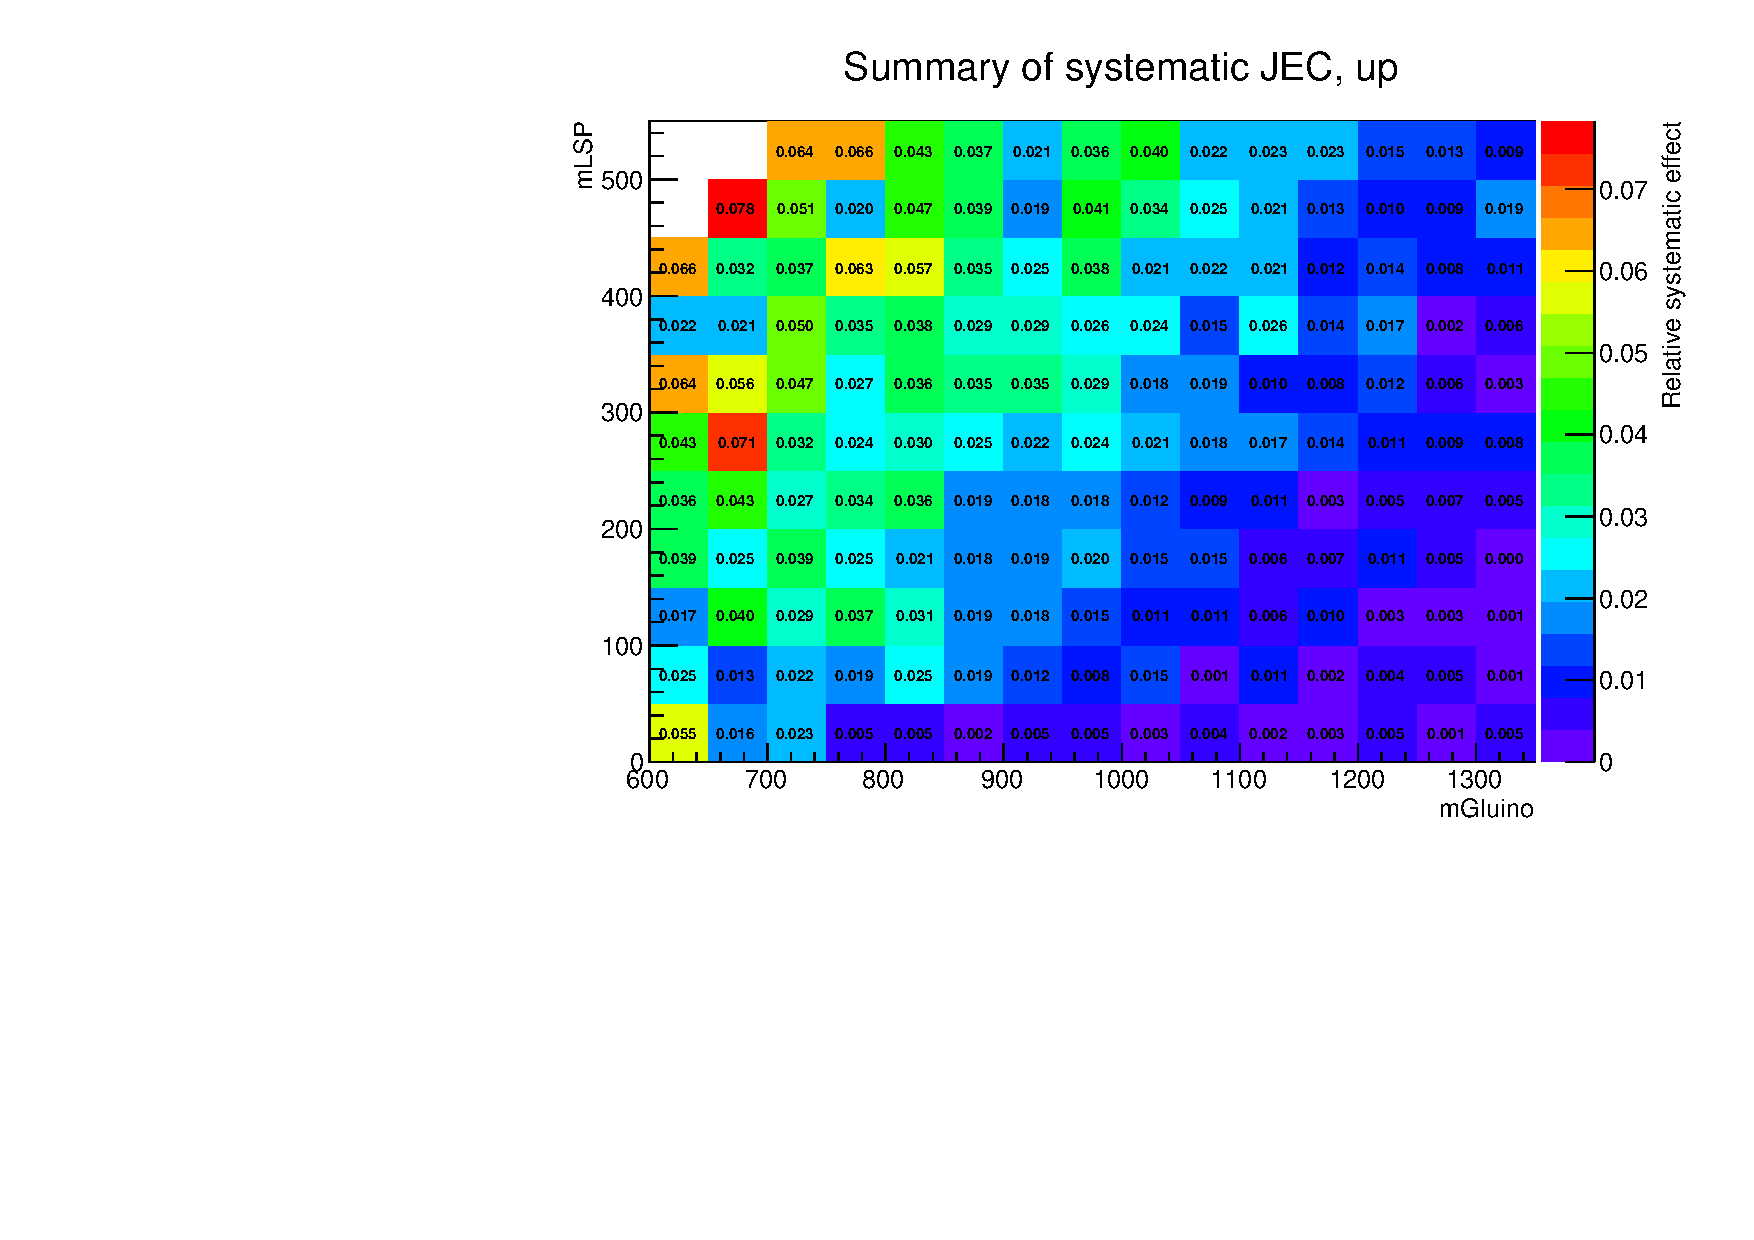
\includegraphics[width=0.49\textwidth]{figures/app_sig_syst/sys_JEC_up}
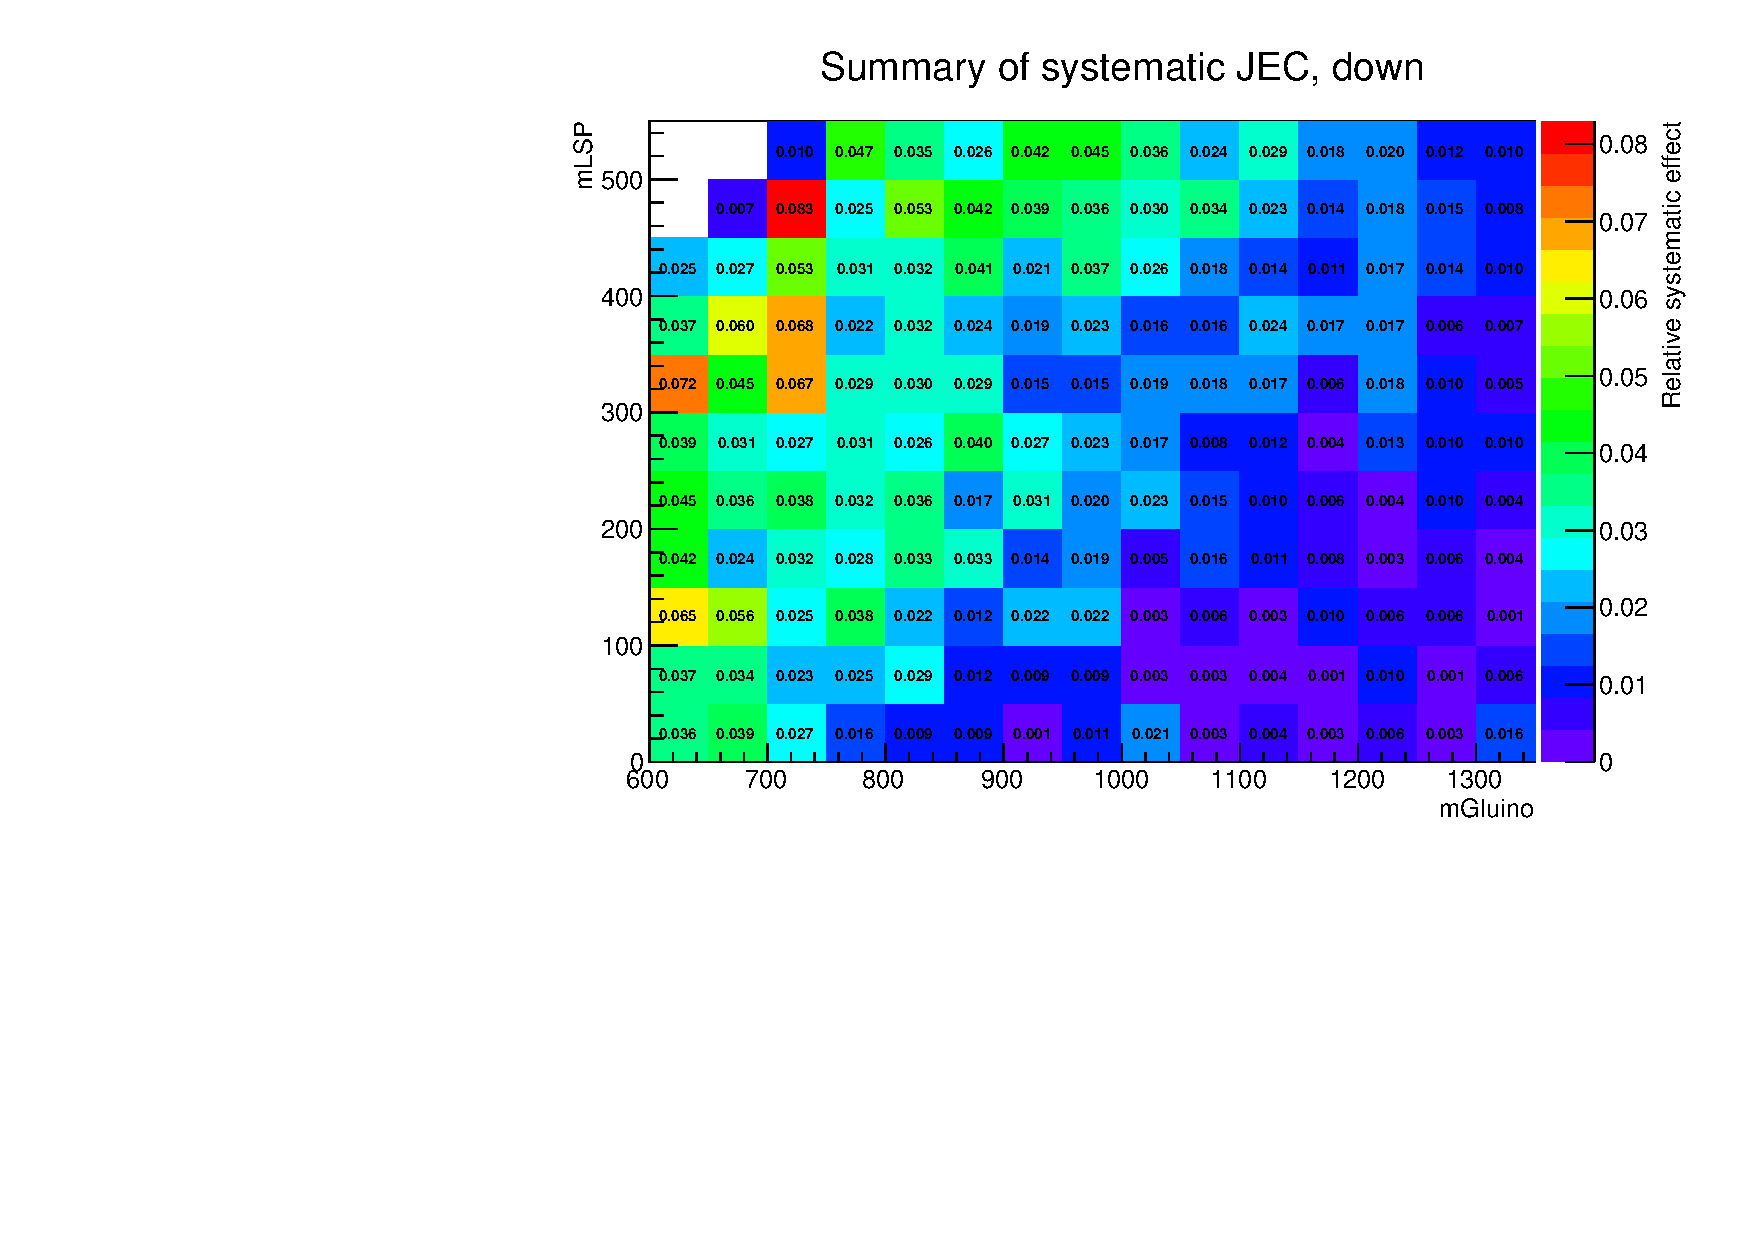
\includegraphics[width=0.49\textwidth]{figures/app_sig_syst/sys_JEC_down}
\caption{$1\sigma$ up (left) and down (right) variation for jet energy corrections.}
\end{figure}

\begin{figure}[htpb]
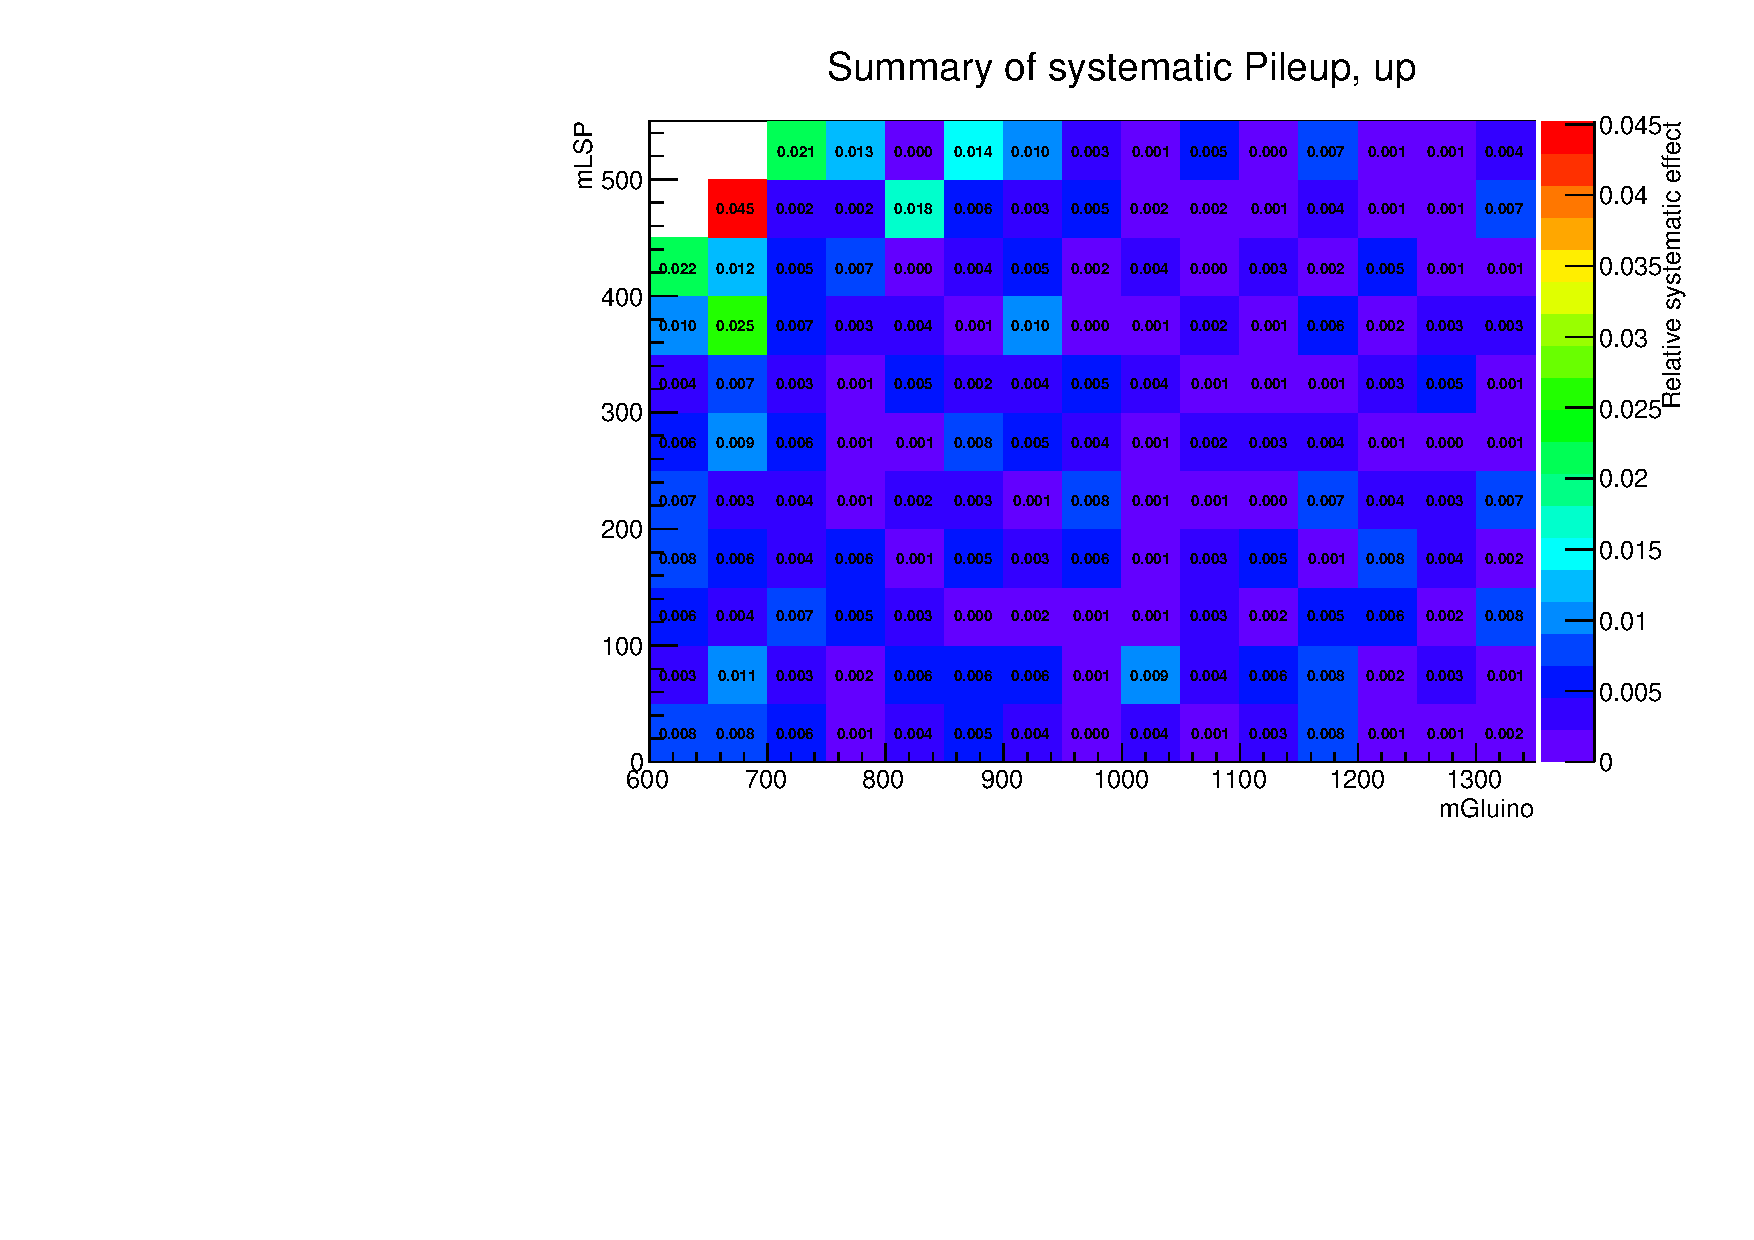
\includegraphics[width=0.49\textwidth]{figures/app_sig_syst/sys_Pileup_up}
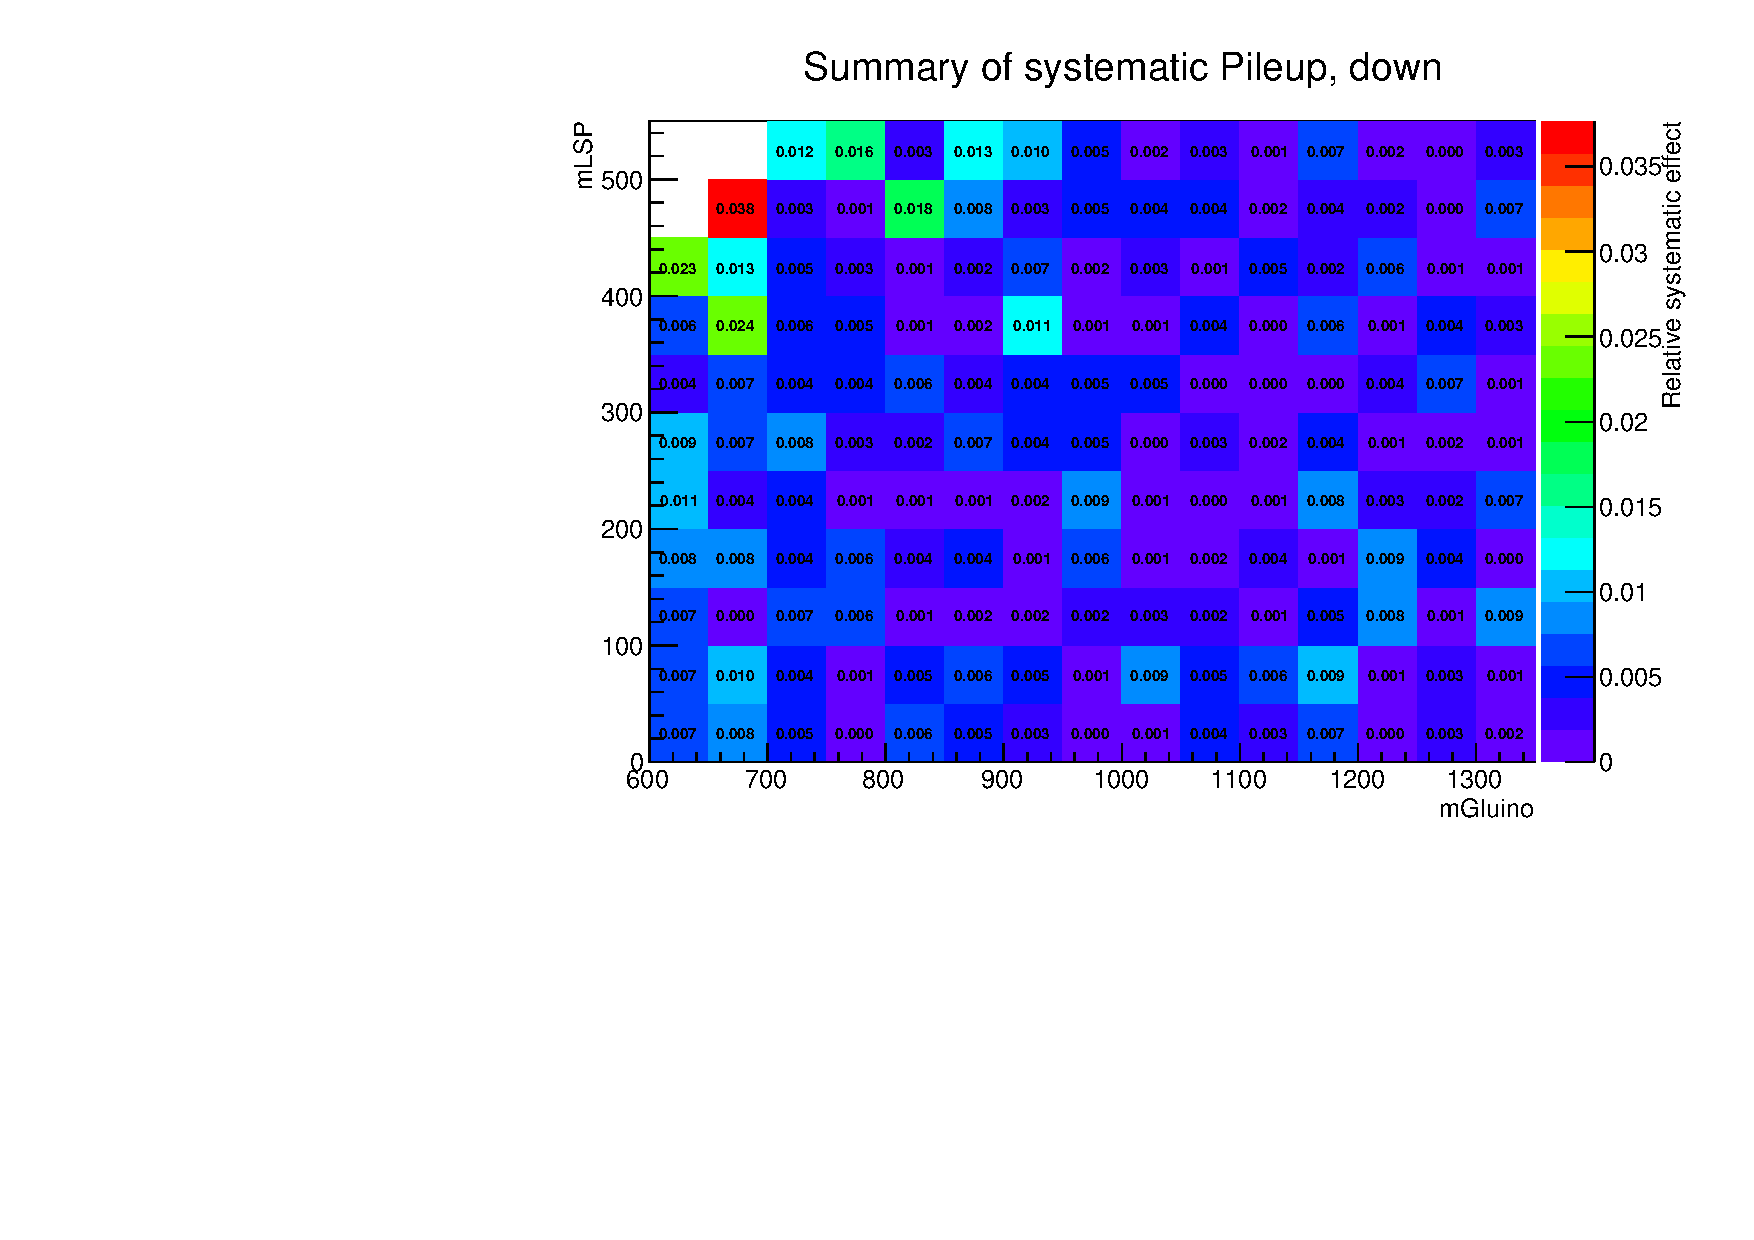
\includegraphics[width=0.49\textwidth]{figures/app_sig_syst/sys_Pileup_down}
\caption{$1\sigma$ up (left) and down (right) variation for pileup reweighting.}
\end{figure}

\begin{figure}[htpb]
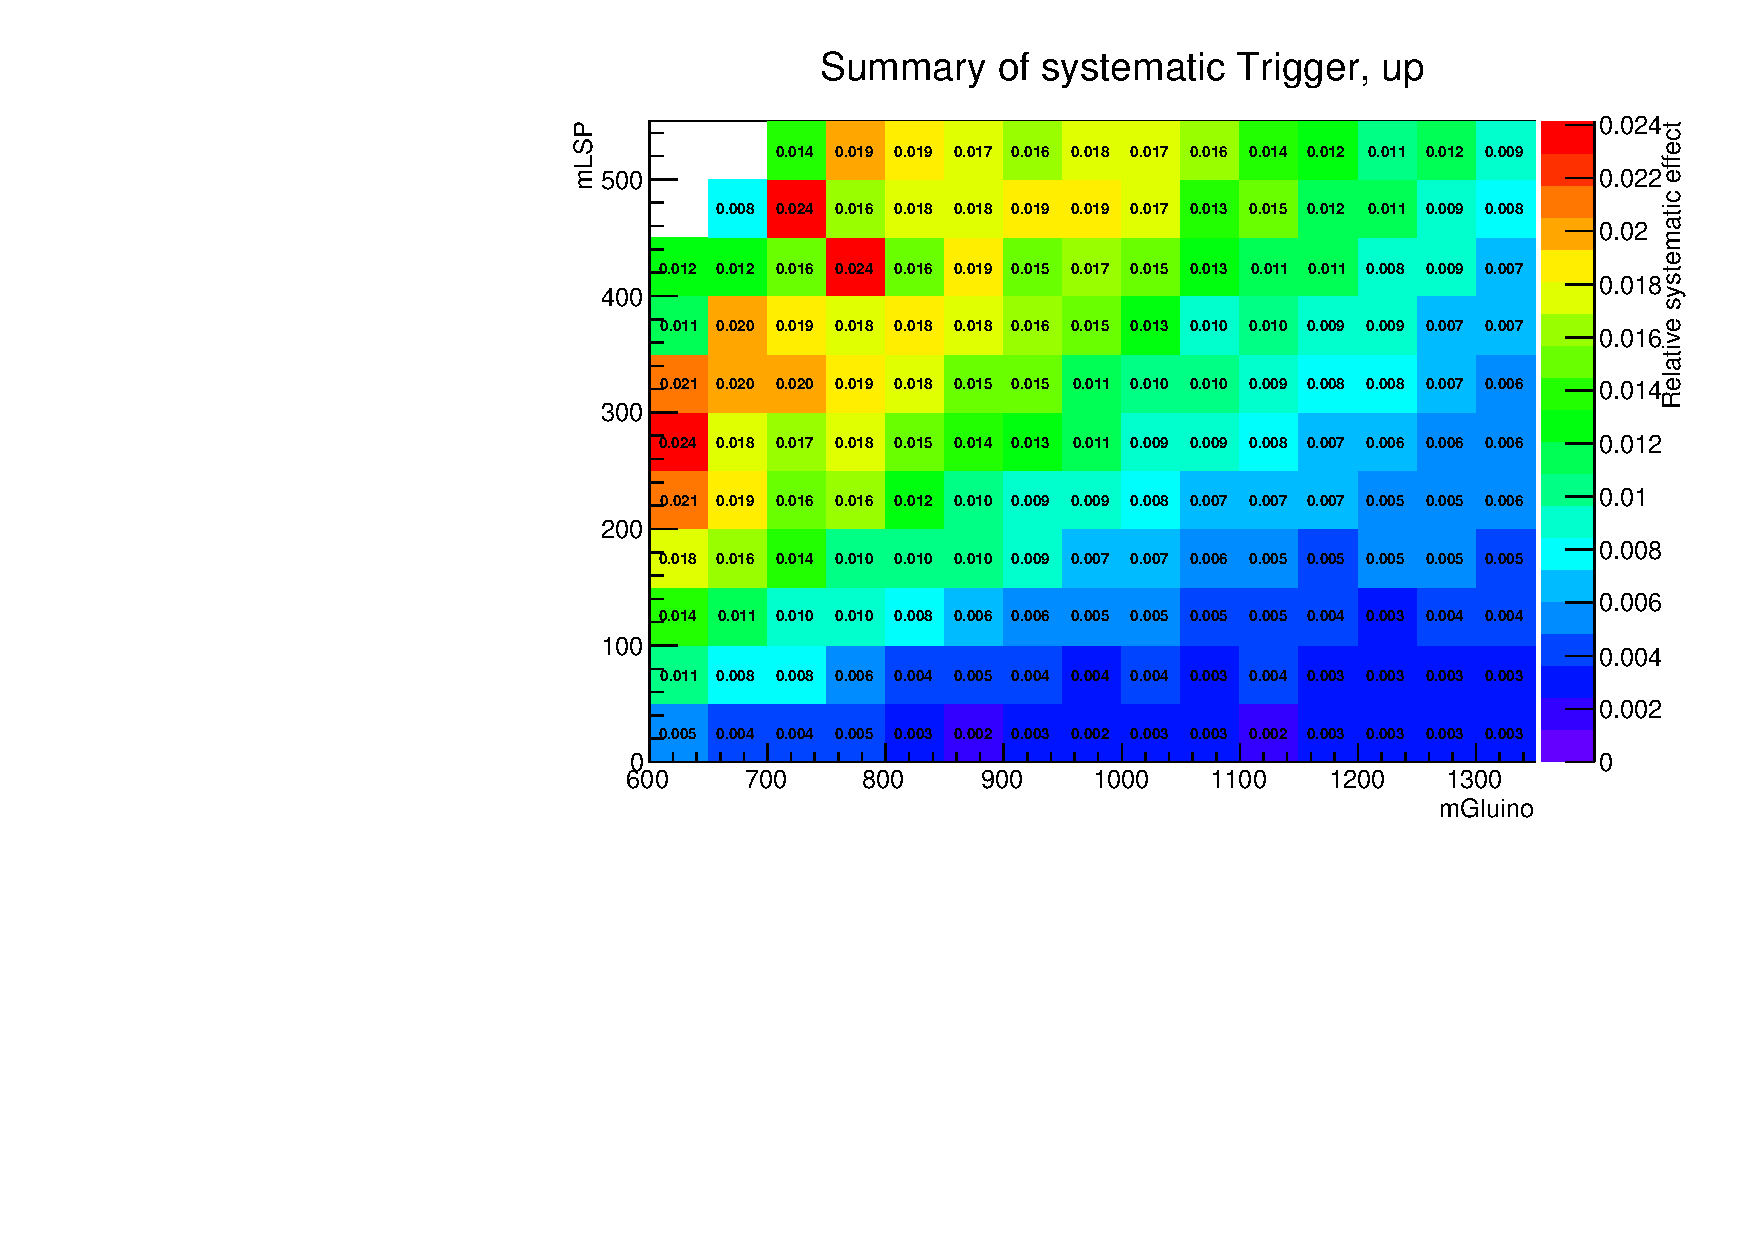
\includegraphics[width=0.49\textwidth]{figures/app_sig_syst/sys_Trigger_up}
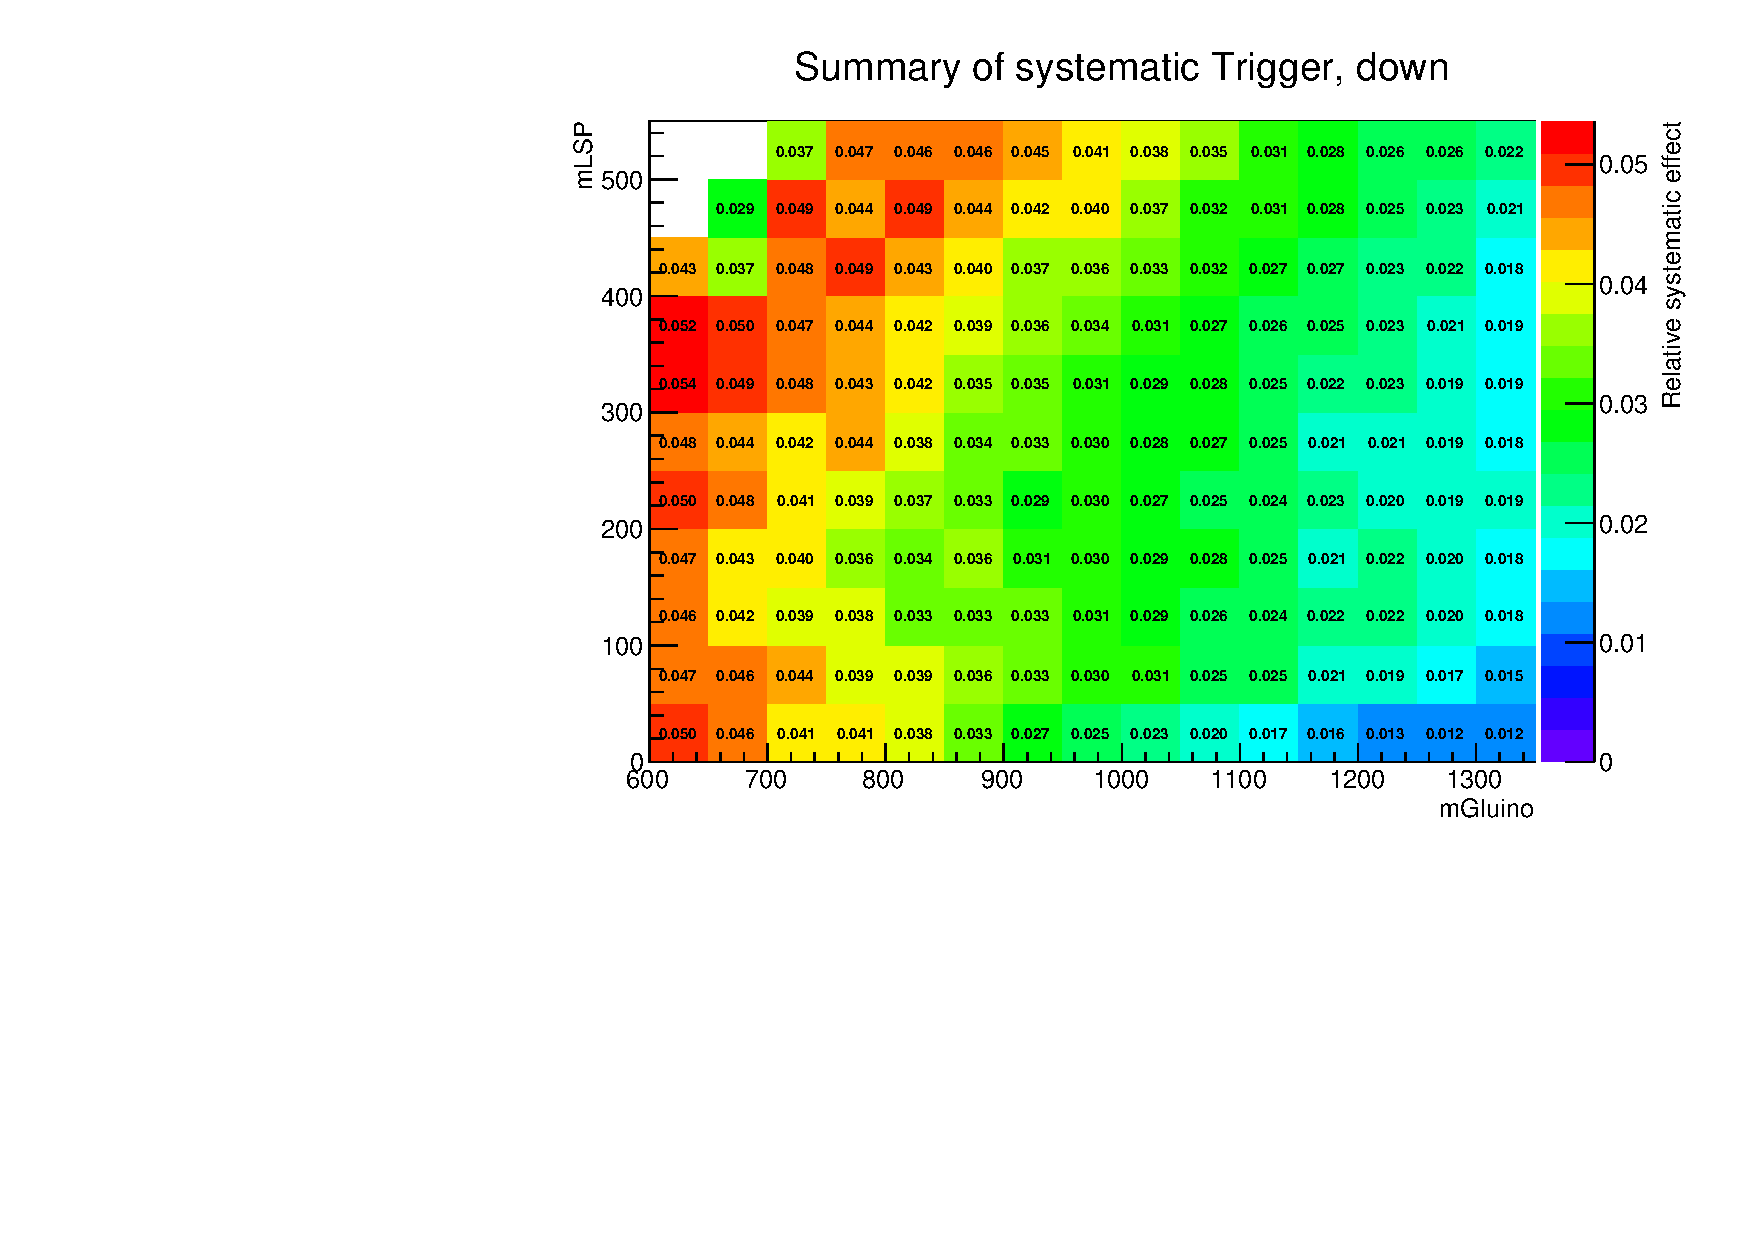
\includegraphics[width=0.49\textwidth]{figures/app_sig_syst/sys_Trigger_down}
\caption{$1\sigma$ up (left) and down (right) variation for trigger efficiency.}
\end{figure}

\begin{figure}[htpb]
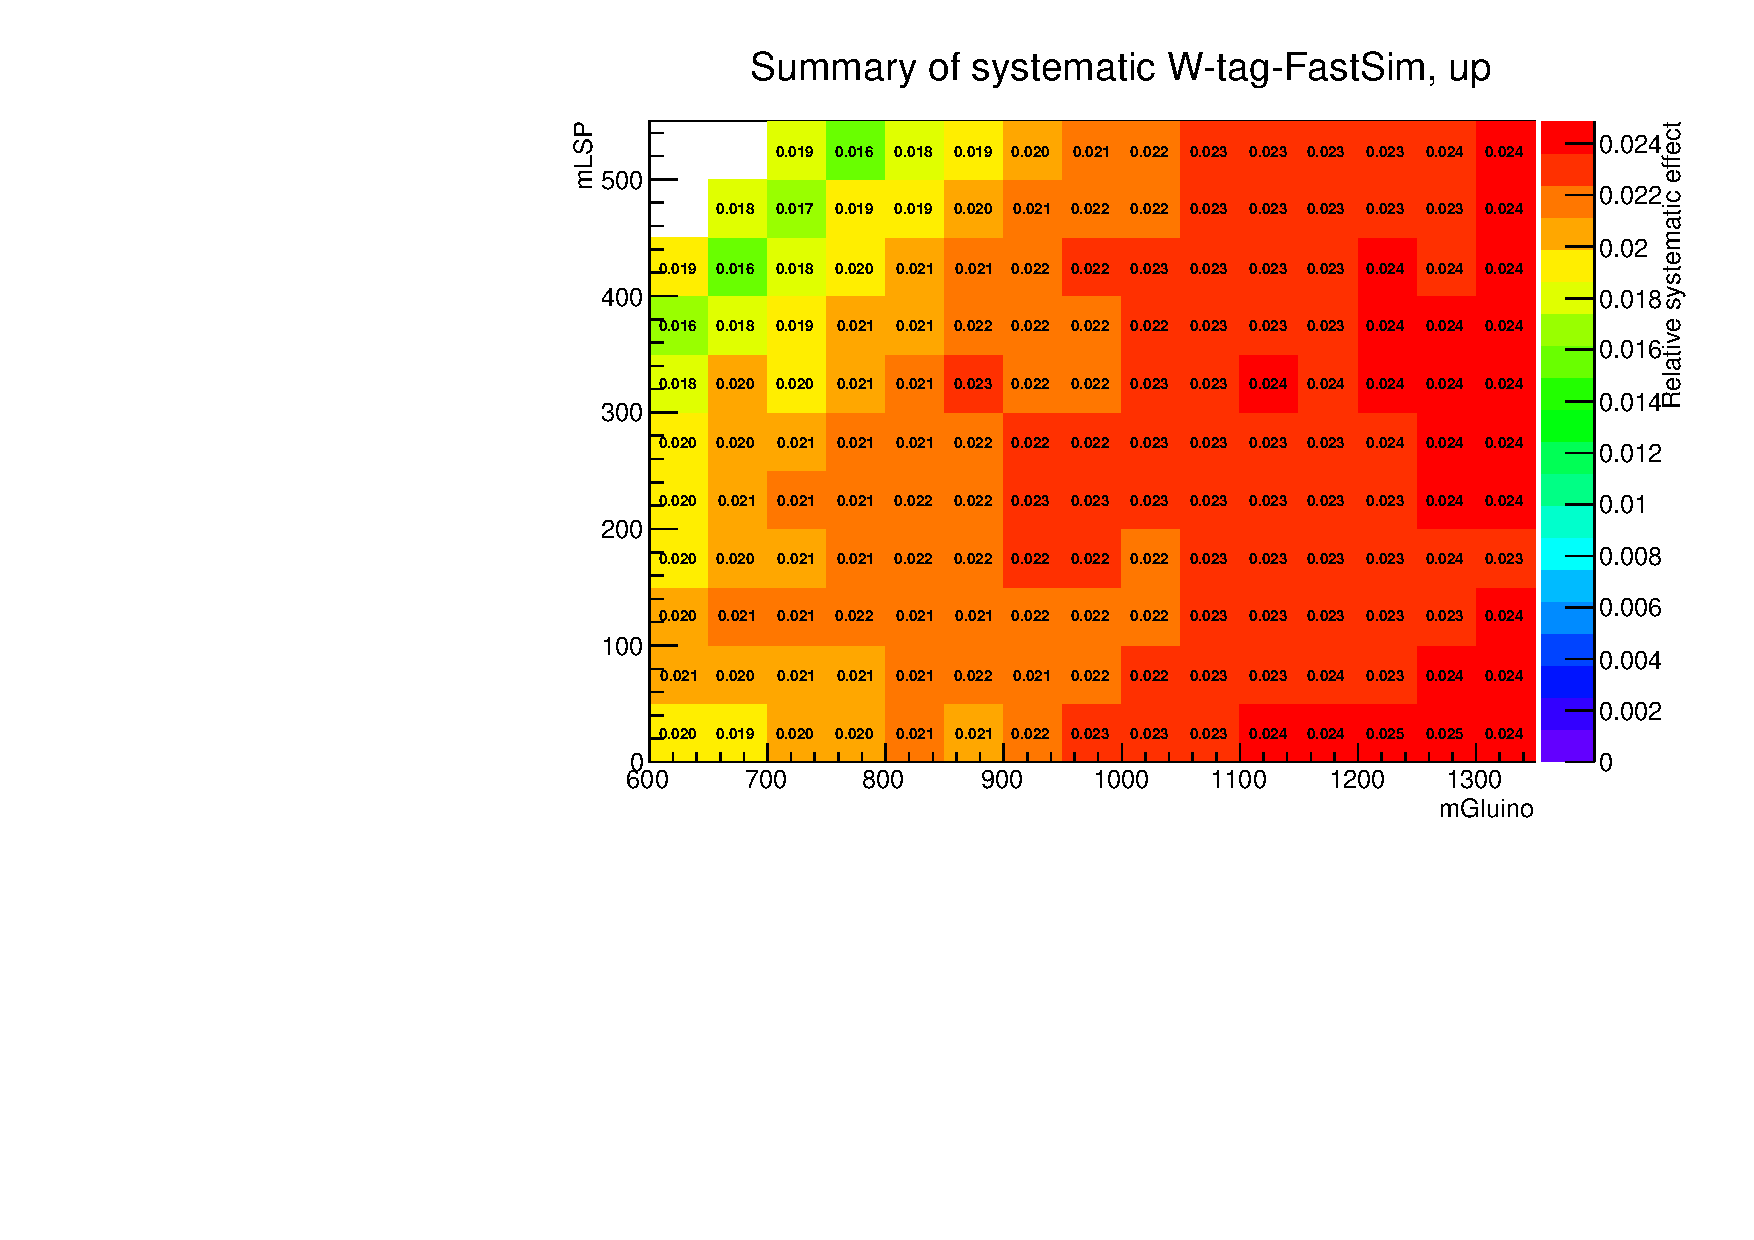
\includegraphics[width=0.49\textwidth]{figures/app_sig_syst/sys_W-tag-FastSim_up}
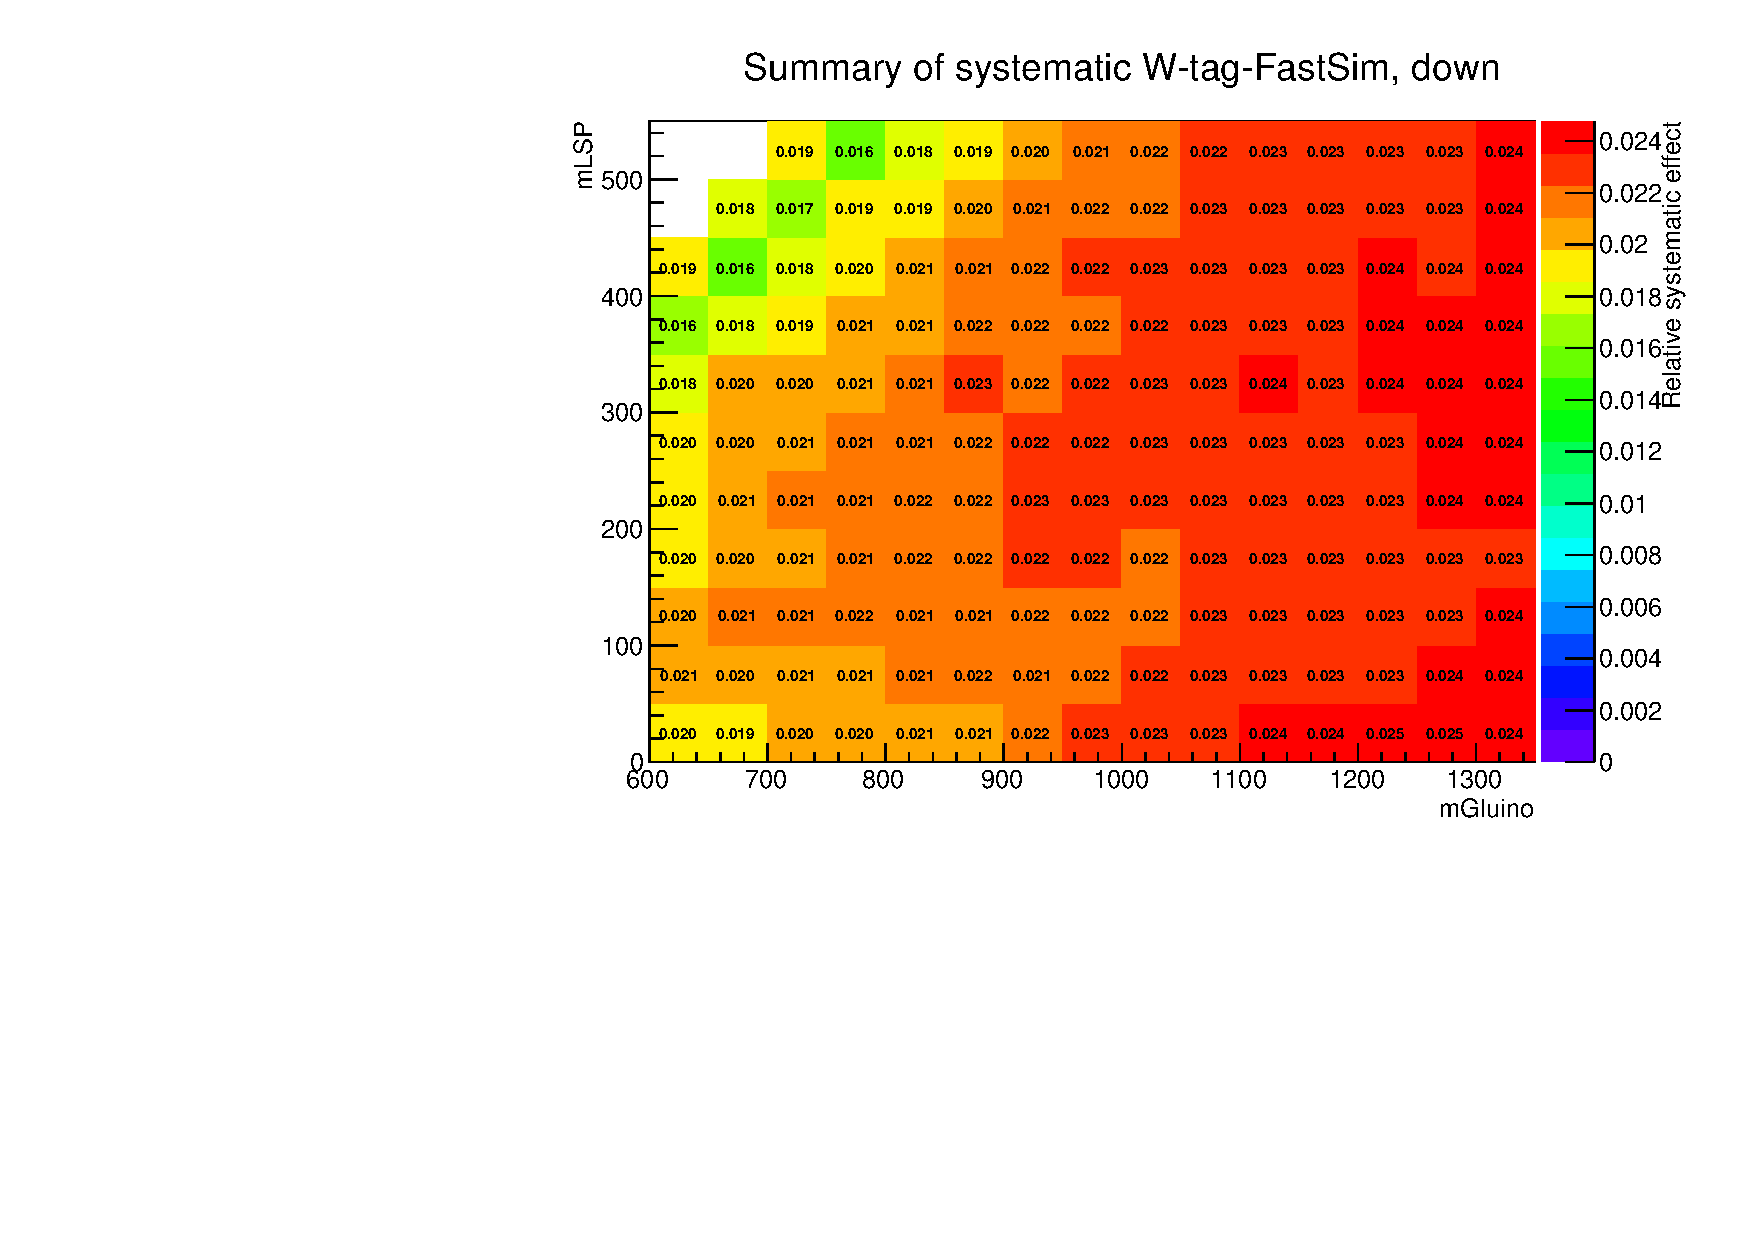
\includegraphics[width=0.49\textwidth]{figures/app_sig_syst/sys_W-tag-FastSim_down}
\caption{$1\sigma$ up (left) and down (right) variation for $\W$ boson tag FullSim/FastSim SF.}
\end{figure}

\begin{figure}[htpb]
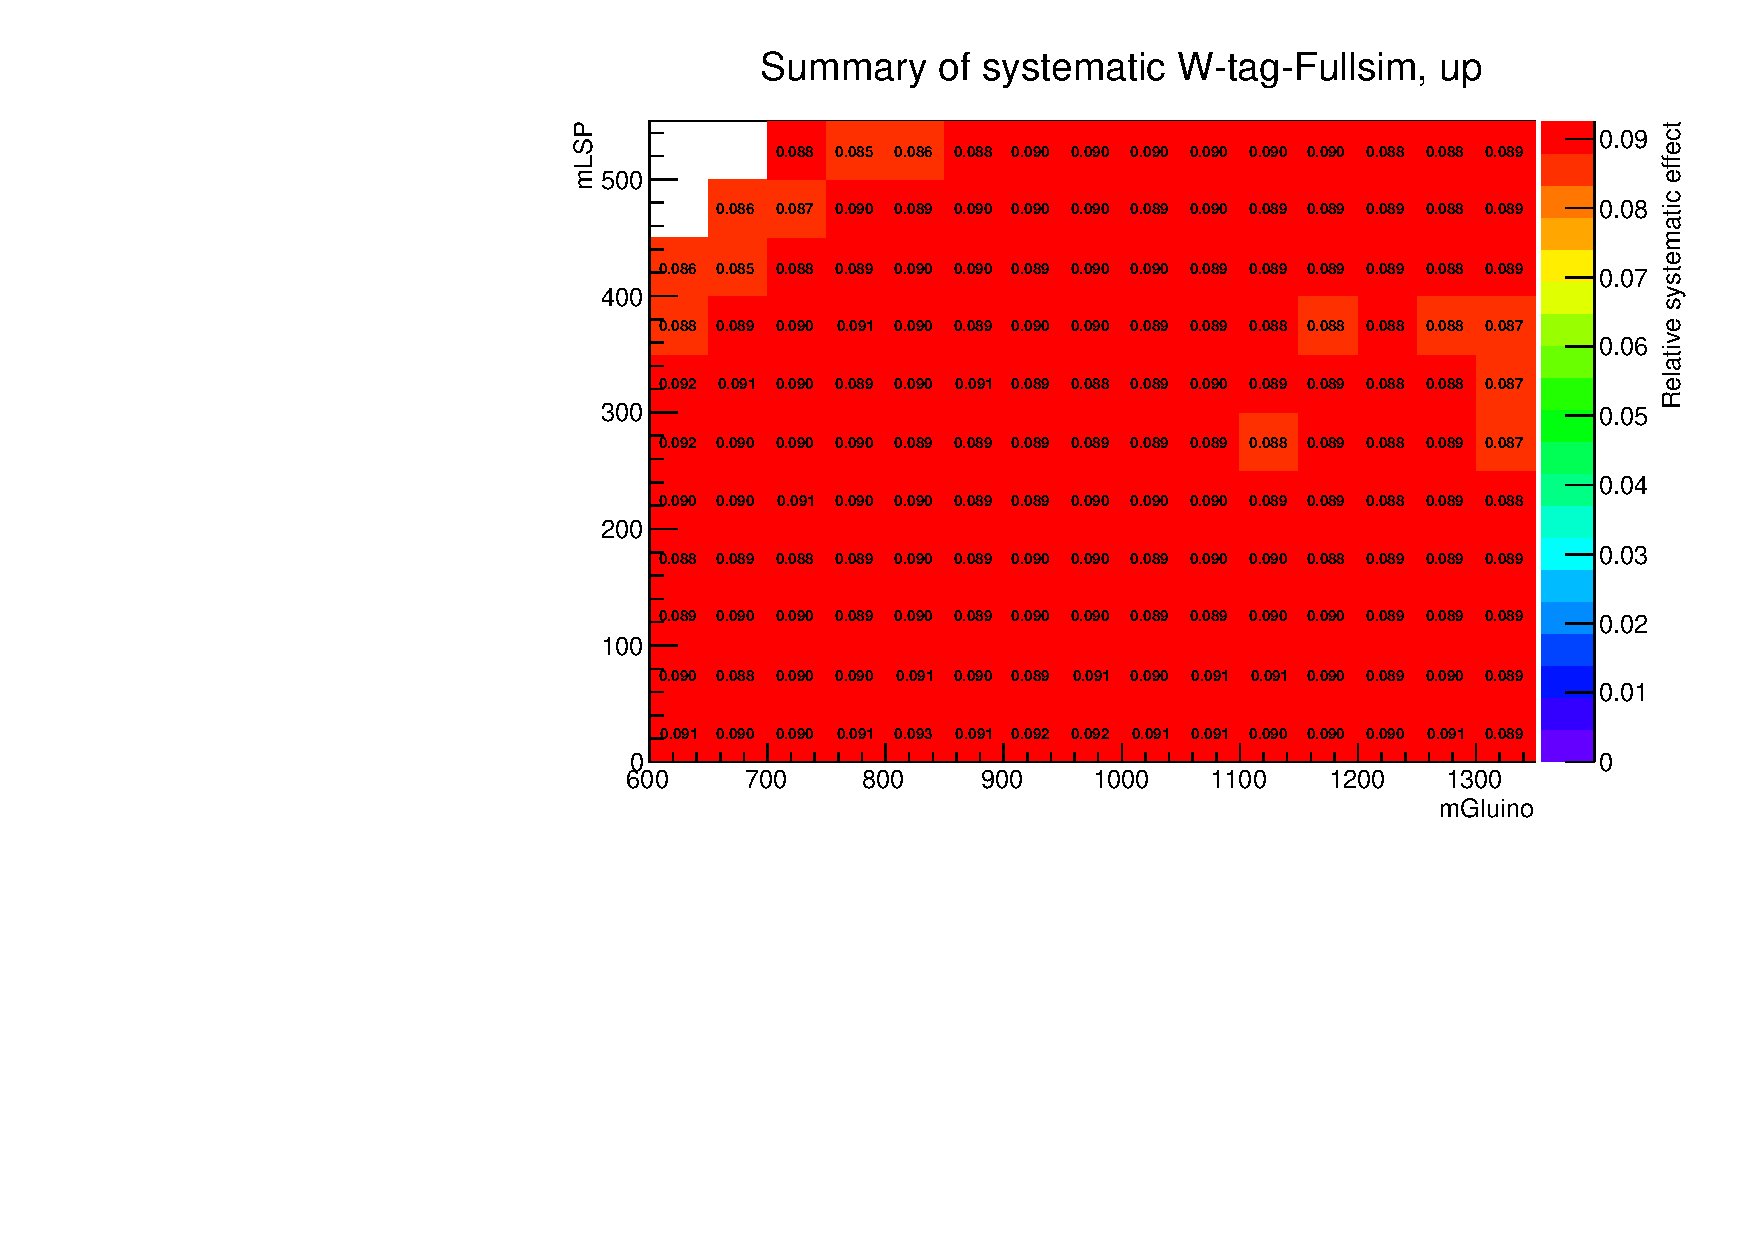
\includegraphics[width=0.49\textwidth]{figures/app_sig_syst/sys_W-tag-Fullsim_up}
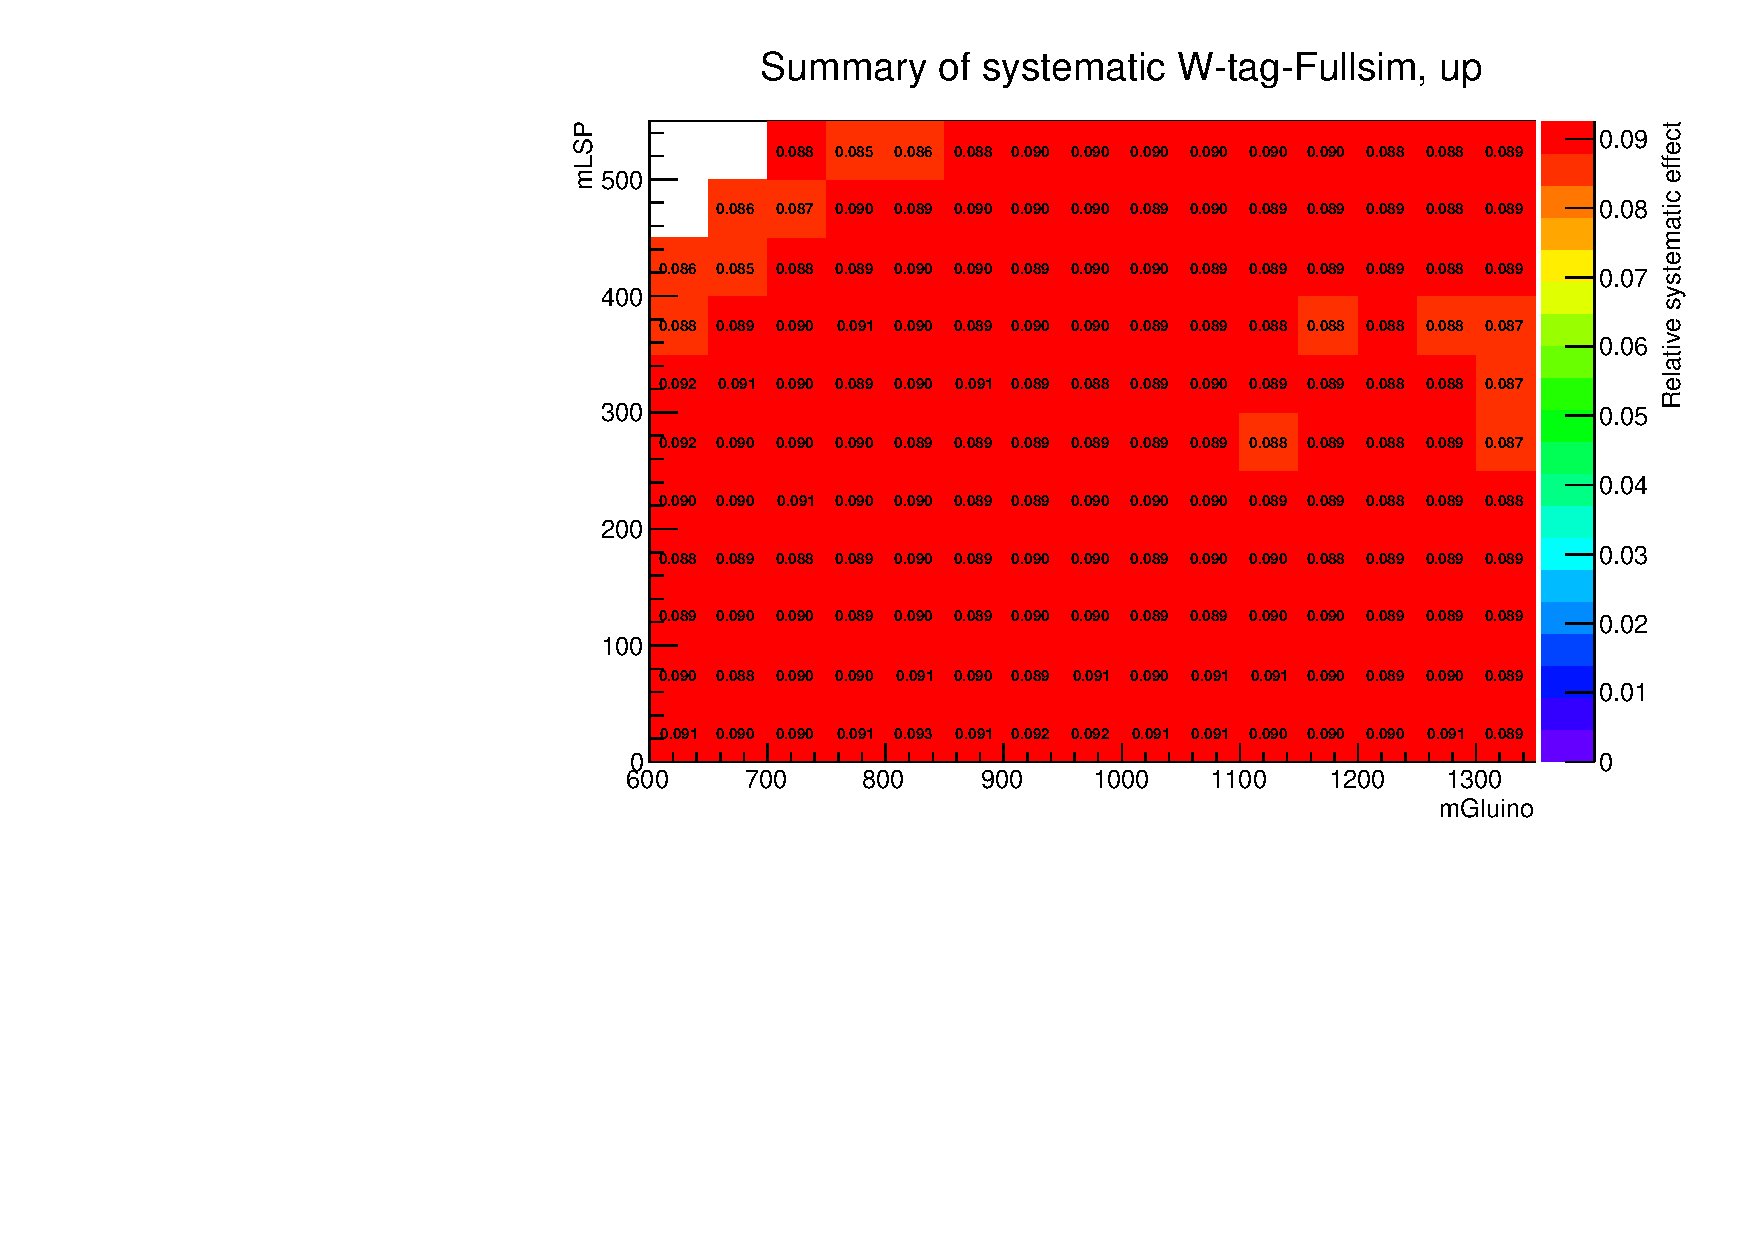
\includegraphics[width=0.49\textwidth]{figures/app_sig_syst/sys_W-tag-Fullsim_up}
\caption{$1\sigma$ up (left) and down (right) variation for $\W$ boson tag Data/FullSim SF.}
\end{figure}

\begin{figure}[htpb]
\centering
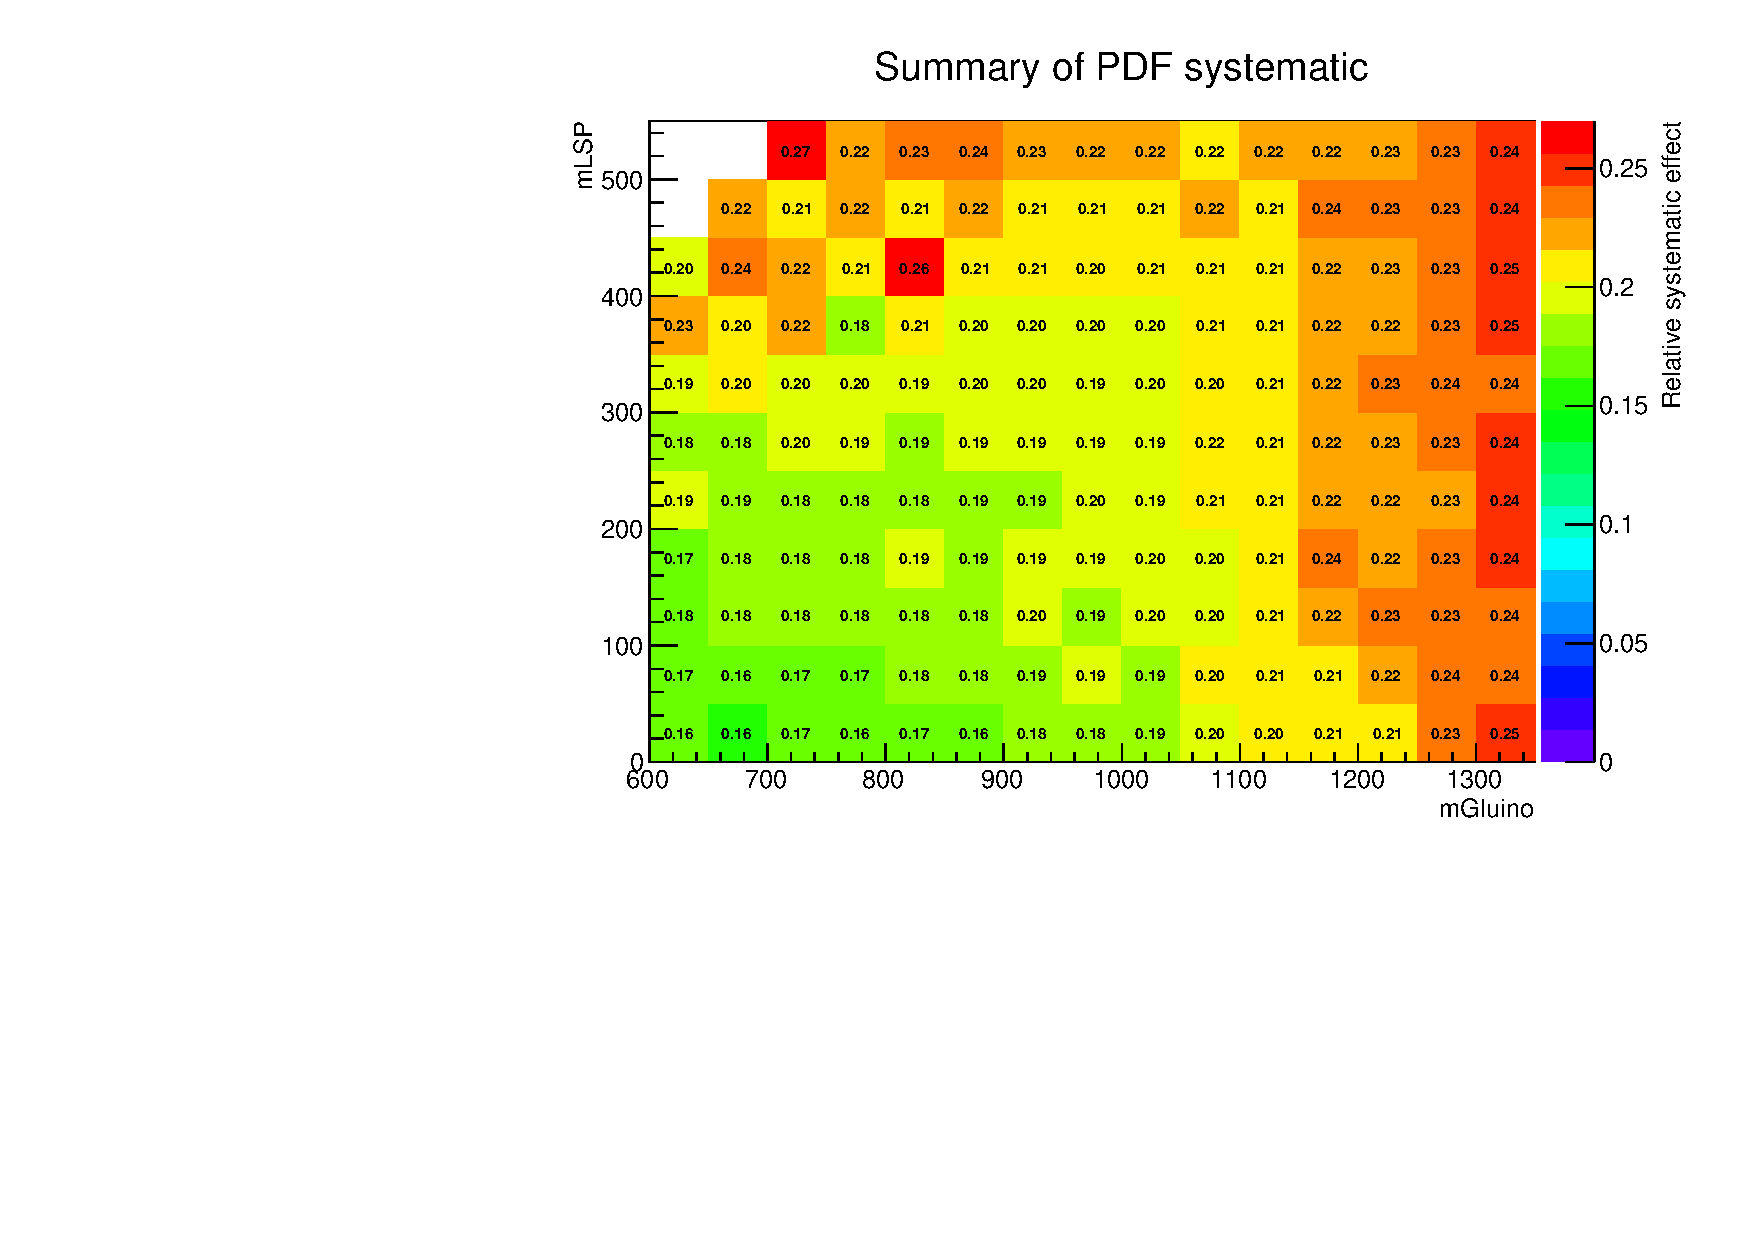
\includegraphics[width=0.49\textwidth]{figures/app_sig_syst/sys_PDF}
\caption{$1\sigma$ variation for the parton distribution functions. \label{fig:sig_sys_end}}
\end{figure}
